%===============================================================================
% LaTeX sjabloon voor de bachelorproef toegepaste informatica aan HOGENT
% Meer info op https://github.com/HoGentTIN/latex-hogent-report
%===============================================================================

\documentclass[dutch,dit,thesis]{hogentreport}

% TODO:
% - If necessary, replace the option `dit`' with your own department!
%   Valid entries are dbo, dbt, dgz, dit, dlo, dog, dsa, soa
% - If you write your thesis in English (remark: only possible after getting
%   explicit approval!), remove the option "dutch," or replace with "english".

\usepackage{lipsum} % For blind text, can be removed after adding actual content
\usepackage{url}

%% Pictures to include in the text can be put in the graphics/ folder
\graphicspath{{../graphics/}}

%% For source code highlighting, requires pygments to be installed
%% Compile with the -shell-escape flag!
%% \usepackage[chapter]{minted}
%% If you compile with the make_thesis.{bat,sh} script, use the following
%% import instead:
\usepackage[chapter]{minted}
\usemintedstyle{solarized-light}

%% Formatting for minted environments.
\setminted{%
    autogobble,
    frame=lines,
    breaklines,
    linenos,
    tabsize=4
}

%% Ensure the list of listings is in the table of contents
\renewcommand\listoflistingscaption{%
    \IfLanguageName{dutch}{Lijst van codefragmenten}{List of listings}
}
\renewcommand\listingscaption{%
    \IfLanguageName{dutch}{Codefragment}{Listing}
}
\renewcommand*\listoflistings{%
    \cleardoublepage\phantomsection\addcontentsline{toc}{chapter}{\listoflistingscaption}%
    \listof{listing}{\listoflistingscaption}%
}

% Other packages not already included can be imported here

%%---------- Document metadata -------------------------------------------------
% TODO: Replace this with your own information
\author{Kyanu Neckebroek}
\supervisor{Dhr. S. Van Impe}
\cosupervisor{Dhr. K. Cools}
\title{Welke machine learning modellen zijn het meest geschikt voor het detecteren van misinformatie op Mastodon en welke inhoudelijke factoren beïnvloeden de nauwkeurigheid van deze modellen?}
\academicyear{\advance\year by -1 \the\year--\advance\year by 1 \the\year}
\examperiod{1}
\degreesought{\IfLanguageName{dutch}{Professionele bachelor in de toegepaste informatica}{Bachelor of applied computer science}}
\partialthesis{false} %% To display 'in partial fulfilment'
%\institution{Internshipcompany BVBA.}

\usepackage{booktabs}
\usepackage{longtable}
\usepackage{array}
\usepackage{xcolor}
\usepackage{listings}
\usepackage{float}
\usepackage{caption}
\usepackage{subcaption}

% Colors and listings style for product documentation
\definecolor{codeblue}{RGB}{33,150,243}
\definecolor{codegray}{RGB}{245,245,245}
\definecolor{codecomment}{RGB}{100,100,100}
\definecolor{codestring}{RGB}{76,175,80}
\definecolor{darkblue}{RGB}{25,100,180}
\definecolor{lightgray}{RGB}{240,240,240}

\lstdefinestyle{pythonstyle}{%
    backgroundcolor=\color{codegray},
    commentstyle=\color{codecomment}\itshape,
    keywordstyle=\color{codeblue}\bfseries,
    stringstyle=\color{codestring},
    basicstyle=\ttfamily\small,
    breakatwhitespace=false,
    breaklines=true,
    captionpos=b,
    keepspaces=true,
    showspaces=false,
    showstringspaces=false,
    showtabs=false,
    tabsize=4,
    frame=single,
    rulecolor=\color{gray!40},
    language=Python
}
\lstset{style=pythonstyle}

\hypersetup{
    colorlinks=true,
    linkcolor=darkblue,
    citecolor=darkblue,
    urlcolor=codeblue,
    pdftitle={Misinformatie Detectie op Mastodon -- Technische Documentatie},
    pdfauthor={}
}

%% Add global exceptions to the hyphenation here
\hyphenation{back-slash}

%% The bibliography (style and settings are  found in hogentthesis.cls)
\addbibresource{bachproef.bib}            %% Bibliography file
\addbibresource{../voorstel/voorstel.bib} %% Bibliography research proposal
\defbibheading{bibempty}{}

%% Prevent empty pages for right-handed chapter starts in twoside mode
\renewcommand{\cleardoublepage}{\clearpage}

\renewcommand{\arraystretch}{1.2}

%% Content starts here.
\begin{document}

%---------- Front matter -------------------------------------------------------

\frontmatter

\hypersetup{pageanchor=false} %% Disable page numbering references
%% Render a Dutch outer title page if the main language is English
\IfLanguageName{english}{%
    %% If necessary, information can be changed here
    \degreesought{Professionele Bachelor toegepaste informatica}%
    \begin{otherlanguage}{dutch}%
       \maketitle%
    \end{otherlanguage}%
}{}

%% Generates title page content
\maketitle
\hypersetup{pageanchor=true}

\documentclass[a4paper,11pt]{report}
\usepackage[dutch]{babel}
\usepackage{geometry}
\usepackage{parskip}
\usepackage{iflang} % Nodig voor \IfLanguageName

\begin{document}

%%=============================================================================
%% Voorwoord
%%=============================================================================

\chapter*{\IfLanguageName{dutch}{Woord vooraf}{Preface}}%
\label{ch:voorwoord}

Voor u ligt de bachelorproef ``Detectie van misinformatie op het decentrale sociale mediaplatform Mastodon'', geschreven als afronding van de opleiding Toegepaste Informatica aan HOGENT.

De keuze voor dit onderwerp vloeit voort uit mijn persoonlijke fascinatie voor de snelle ontwikkelingen binnen Artificial Intelligence en de impact hiervan op onze samenleving. In een tijd waarin sociale media vaak onder vuur liggen vanwege polarisatie en nepnieuws, trok de opkomst van het `Fediverse' en Mastodon mijn aandacht. Het leek mij een uitdagend technisch en maatschappelijk vraagstuk: hoe houden we een platform schoon zonder centrale autoriteit?

Het schrijven van deze scriptie en het bouwen van de bijbehorende modellen was een leerzaam proces. Het heeft mij niet alleen dieper inzicht gegeven in Natural Language Processing en modellen zoals BERT, maar ook in de complexiteit van dataverzameling op een decentraal netwerk.

Graag wil ik iedereen bedanken die mij tijdens dit traject heeft gesteund. In de eerste plaats wil ik mijn promotor, lector Steven Van Impe, en mijn co-promotor, Kasper Cools, bedanken voor de waardevolle feedback en het sturen van mijn onderzoek in de juiste richting. Ook gaat mijn dank uit naar de docenten van de specialisatie AI \& Data Engineering voor de stevige basis die zij mij de afgelopen jaren hebben meegegeven.

Tot slot wil ik mijn ouders en vrienden bedanken. Hun geduld, aanmoedigingen en de nodige ontspanning tijdens de drukke periodes waren onmisbaar om dit project tot een goed einde te brengen.

\vspace{1cm}

Kyanu Neckebroek \\
Gent, mei 2026

\end{document}
%%=============================================================================
%% Samenvatting
%%=============================================================================

% TODO: De "abstract" of samenvatting is een kernachtige (~ 1 blz. voor een
% thesis) synthese van het document.
%
% Een goede abstract biedt een kernachtig antwoord op volgende vragen:
%
% 1. Waarover gaat de bachelorproef?
% 2. Waarom heb je er over geschreven?
% 3. Hoe heb je het onderzoek uitgevoerd?
% 4. Wat waren de resultaten? Wat blijkt uit je onderzoek?
% 5. Wat betekenen je resultaten? Wat is de relevantie voor het werkveld?
%
% Daarom bestaat een abstract uit volgende componenten:
%
% - inleiding + kaderen thema
% - probleemstelling
% - (centrale) onderzoeksvraag
% - onderzoeksdoelstelling
% - methodologie
% - resultaten (beperk tot de belangrijkste, relevant voor de onderzoeksvraag)
% - conclusies, aanbevelingen, beperkingen
%
% LET OP! Een samenvatting is GEEN voorwoord!

%%---------- Nederlandse samenvatting -----------------------------------------
%
% TODO: Als je je bachelorproef in het Engels schrijft, moet je eerst een
% Nederlandse samenvatting invoegen. Haal daarvoor onderstaande code uit
% commentaar.
% Wie zijn bachelorproef in het Nederlands schrijft, kan dit negeren, de inhoud
% wordt niet in het document ingevoegd.

\IfLanguageName{english}{%
\selectlanguage{dutch}
\chapter*{Samenvatting}
\lipsum[1-4]
\selectlanguage{english}
}{}

%%---------- Samenvatting -----------------------------------------------------
% De samenvatting in de hoofdtaal van het document

\chapter*{\IfLanguageName{dutch}{Samenvatting}{Abstract}}

Deze bachelorproef onderzoekt de detectie van misinformatie op Mastodon, een gedecentraliseerd sociaal netwerk zonder centrale moderatie. Het onderzoek stelt de vraag welke machine learning modellen het meest geschikt zijn om misleidende berichten te classificeren op Mastodon en welke inhoudelijke factoren de nauwkeurigheid van die modellen beïnvloeden.

De methodologie combineert een aangepaste versie van de LIAR-dataset met 300 Mastodon-berichten die ik handmatig heb gelabeld. Voor de traditionele modellen (Logistic Regression en Support Vector Machines) werden tekstfuncties omgezet met TF-IDF, terwijl het Transformer-gebaseerde BERT-model werd gefinetuned op dezelfde dataset. Evaluatie is uitgevoerd op een onafhankelijke testset met standaard metrieken zoals accuracy, macro F1, precision, recall en AUC-ROC.

De resultaten tonen gemengde bevindingen: BERT bereikt de hoogste accuracy (0,652), de hoogste macro F1-score (0,638), de hoogste binaire F1-score (0,709) en de hoogste AUC-ROC (0,682). Logistic Regression blijft een sterke baseline met vergelijkbare prestaties (accuracy 0,639, macro F1 0,633), terwijl SVM beduidend lager presteert (accuracy 0,622, macro F1 0,576) ondanks het hoogste recall voor de klasse "waar" (0,830). BERT wordt als meest geschikt aangemerkt omdat: (1) het allround de beste evaluatiecijfers heeft, (2) het beter generaliseert op nieuwe, onbekende berichten, (3) de macro F1-score het model robuust maakt over beide klassen, en (4) het consistent goed presteert in zowel precieze als recall-gevoelige toepassingen. Logistic Regression blijft waardevol als snelle, transparante baseline die met minimale computerbronnen kan draaien.

Verder onderzoek naar inhoudelijke factoren laat zien dat langere berichten en berichten met lage bronbetrouwbaarheid vaker tot classificatiefouten leiden. Taalgebruikkenmerken zoals vraagtekens, hoofdletters en URLs blijken eveneens invloedrijk voor de modelprestaties, wat aangeeft dat zowel tekstinhoud als stijlkenmerken belangrijke signalen bevatten.

De conclusie is dat BERT in deze experimentele opzet de meest geschikte basis biedt voor automatische detectie van misinformatie op Mastodon, maar dat een hybride aanpak met traditionele modellen en menselijke moderatie realistischer is vanwege de fragmentatie en variatie in Mastodon-data. Aanbevolen wordt de dataset uit te breiden en contextuele kenmerken verder te integreren om de betrouwbaarheid van de detectiesysteem verder te verhogen.


%---------- Inhoud, lijst figuren, ... -----------------------------------------

\tableofcontents

% In a list of figures, the complete caption will be included. To prevent this,
% ALWAYS add a short description in the caption!
%
%  \caption[short description]{elaborate description}
%
% If you do, only the short description will be used in the list of figures

\listoffigures

% If you included tables and/or source code listings, uncomment the appropriate
% lines.
\listoftables

\listoflistings

% Als je een lijst van afkortingen of termen wil toevoegen, dan hoort die
% hier thuis. Gebruik bijvoorbeeld de ``glossaries'' package.
% https://www.overleaf.com/learn/latex/Glossaries

%---------- Kern ---------------------------------------------------------------

\mainmatter

% 1. Inleiding
\IfFileExists{inleiding.tex}{
    \documentclass[a4paper,11pt]{report}
\usepackage[dutch]{babel}
\usepackage{geometry}
\usepackage{parskip}

% Dit is een opzet zodat je de tekst hier als PDF kunt bekijken.
% Voor je eigen thesis: kopieer alles hieronder (vanaf \chapter) naar je eigen bestand.

\begin{document}

\chapter{Inleiding}
\label{ch:inleiding}

De verspreiding van misinformatie op sociale media wordt beschouwd als een van de grootste uitdagingen van het digitale tijdperk. Terwijl platformen zoals Facebook (Meta) en X (voorheen Twitter) zwaar investeren in gecentraliseerde moderatie-algoritmen en factchecking-partnerships, vindt er een verschuiving plaats in het sociale medialandschap. Een groeiend aantal gebruikers migreert naar het ``Fediverse'', met Mastodon als de meest prominente speler.

Mastodon onderscheidt zich door zijn decentrale architectuur: er is geen centrale eigenaar, geen centraal algoritme en—cruciaal voor dit onderzoek—geen centraal moderatieteam. Elke server (instantie) wordt beheerd door vrijwilligers die verantwoordelijk zijn voor hun eigen regels. Dit creëert een unieke uitdaging: hoe kan misinformatie effectief gedetecteerd worden in een omgeving waar data gefragmenteerd is en moderatoren vaak overbelast zijn?

Dit onderzoek richt zich op de toepasbaarheid van machine learning (ML) voor het ondersteunen van deze moderatoren. Specifiek wordt onderzocht of geavanceerde taalmodellen zoals BERT een significant voordeel bieden ten opzichte van traditionele classificatiemethoden in de specifieke context van Mastodon-berichten (``toots'').

\section{Probleemstelling}
\label{sec:probleemstelling}

De huidige tools voor automatische detectie van misinformatie zijn voornamelijk ontwikkeld voor en getraind op data van gecentraliseerde platformen zoals X en Reddit. Deze modellen leunen vaak op metadata die specifiek is voor die platformen (zoals globale like-counts of geverifieerde vinkjes) of gaan uit van een uniforme dataset.

Op Mastodon is de situatie fundamenteel anders. Berichten kunnen langer zijn (vaak 500 tekens in plaats van 280), de metadata verschilt per instantie, en de verspreiding van berichten verloopt via een federatief protocol (ActivityPub). Een model dat getraind is op korte tweets presteert mogelijk suboptimaal op de rijkere context van Mastodon-posts. Bovendien hebben beheerders van kleinere Mastodon-instanties vaak niet de middelen om dure, commerciële moderatietools in te kopen.

De doelgroep van dit onderzoek bestaat primair uit **beheerders en moderatoren van Mastodon-instanties**. Zij hebben behoefte aan open-source, toegankelijke inzichten over welke detectiemethoden effectief zijn om hun lokale tijdlijnen schoon te houden. Daarnaast is dit onderzoek relevant voor **onderzoekers in data science en media**, die inzicht willen krijgen in hoe desinformatie zich gedraagt op decentrale netwerken.

\section{Onderzoeksvraag}
\label{sec:onderzoeksvraag}

Het doel van deze bachelorproef is om te bepalen welk type machine learning model het meest geschikt is voor de detectie van misinformatie binnen de technische en inhoudelijke context van Mastodon. De hoofdonderzoeksvraag luidt als volgt:

\begin{quote}
    \textit{In hoeverre presteert het Transformer-gebaseerde model BERT beter in het detecteren van misinformatie op Mastodon in vergelijking met traditionele machine learning modellen zoals Support Vector Machines en Logistic Regression?}
\end{quote}

Om deze vraag te beantwoorden, worden de volgende deelvragen gehanteerd:
\begin{enumerate}
    \item Wat is de invloed van platform-specifieke kenmerken van Mastodon (zoals berichtlengte en decentrale metadata) op de nauwkeurigheid van de modellen?
    \item Welke performantie (uitgedrukt in F1-score, precision en recall) behalen de modellen wanneer ze getraind worden op de algemene LIAR-dataset en toegepast worden op Mastodon-specifieke data?
    \item Is de computationele meerkost van een zwaar model als BERT te verantwoorden voor de behaalde accuratessewinst ten opzichte van lichtere modellen?
\end{enumerate}

\section{Onderzoeksdoelstelling}
\label{sec:onderzoeksdoelstelling}

Het beoogde resultaat van deze bachelorproef is een **vergelijkende studie** ondersteund door een **technische proof-of-concept**.

De criteria voor succes zijn:
\begin{itemize}
    \item Het opleveren van een gelabelde dataset van minimaal 500 Mastodon-berichten (gebaseerd op factchecks).
    \item Een werkende implementatie van drie modellen (Logistic Regression, SVM, BERT) die getraind en getest zijn op deze data.
    \item Een kwantitatieve evaluatie waarbij de F1-scores van de modellen tegen elkaar worden afgezet.
    \item Een adviesrapport voor moderatoren over de haalbaarheid van automatische detectie op hun instanties.
\end{itemize}

Het doel is niet om een volledig productie-klaar moderatieplatform te bouwen, maar om de effectiviteit van de onderliggende detectie-algoritmen te valideren.

\section{Opzet van deze bachelorproef}
\label{sec:opzet-bachelorproef}

De rest van deze bachelorproef is als volgt opgebouwd:

In Hoofdstuk~\ref{ch:stand-van-zaken} wordt een overzicht gegeven van de stand van zaken binnen het onderzoeksdomein. Hierbij wordt dieper ingegaan op de werking van het Mastodon-netwerk, de huidige state-of-the-art in fake news detectie en de theoretische achtergrond van de gebruikte algoritmen (SVM, BERT).

In Hoofdstuk~\ref{ch:methodologie} wordt de methodologie toegelicht. Dit omvat het proces van dataverzameling via de Mastodon API, de pre-processing stappen van de LIAR-dataset en de configuratie van de getrainde modellen.

In Hoofdstuk~\ref{ch:resultaten} worden de experimentele resultaten gepresenteerd. De performantie van de verschillende modellen wordt vergeleken aan de hand van verwarringsmatrices en statistische metrieken. Ook wordt een foutenanalyse uitgevoerd op de incorrect geclassificeerde berichten.

In Hoofdstuk~\ref{ch:conclusie}, tenslotte, wordt de conclusie gegeven en een antwoord geformuleerd op de onderzoeksvragen. Daarbij wordt ook een aanzet gegeven voor toekomstig onderzoek, zoals de integratie van dergelijke modellen in live moderatie-bots.

\end{document}
}{
    \chapter{Inleiding}
    \textit{Let op: bestand inleiding.tex niet gevonden.}
}

% 2. Stand van zaken (Nog te doen)
% !TeX root = NeckebroekKyanuBP.tex
\chapter{\IfLanguageName{dutch}{Stand van zaken}{State of the art}}%
\label{ch:stand-van-zaken}

% Tip: Begin elk hoofdstuk met een paragraaf inleiding die beschrijft hoe
% dit hoofdstuk past binnen het geheel van de bachelorproef. Geef in het
% bijzonder aan wat de link is met het vorige en volgende hoofdstuk.

% Pas na deze inleidende paragraaf komt de eerste sectiehoofding.

Dit hoofdstuk biedt een uitgebreid overzicht van de wetenschappelijke literatuur rond de detectie van misinformatie op sociale media, met een specifieke focus op het gedecentraliseerde platform Mastodon. Omdat Mastodon een relatief nieuw fenomeen is in de academische wereld, zal eerst een breed kader worden geschetst van misinformatie op traditionele sociale media, waarna de specifieke context van het Fediverse wordt diepgravend wordt geanalyseerd.

Het hoofdstuk is als volgt opgebouwd:
\begin{enumerate}
    \item \textbf{Misinformatie en Desinformatie:} Definities, types, en de psychologie achter waarom mensen het delen.
    \item \textbf{Het Fediverse en Mastodon:} De technische architectuur (ActivityPub), de specifieke moderatie-uitdagingen en de verschillen met platformen als X (Twitter).
    \item \textbf{Automatische Detectie:} Een diepgaande vergelijking tussen traditionele feature-based methoden (zoals SVM) en moderne deep learning methoden (zoals BERT).
    \item \textbf{Datasets en Benchmarking:} Een analyse van bestaande datasets zoals LIAR en de noodzaak voor domeinspecifieke data.
\end{enumerate}

\section{Misinformatie en Desinformatie: Een Conceptueel Kader}
\label{sec:misinformatie-definitie}

In het huidige digitale tijdperk is de verspreiding van onjuiste informatie uitgegroeid tot een van de grootste maatschappelijke uitdagingen. Hoewel de termen ``fake news'', ``misinformatie'' en ``desinformatie'' vaak door elkaar worden gebruikt in het publieke debat, hanteren wetenschappers strikte definities om de nuances van dit probleem te vatten. Het invloedrijke raamwerk van \textcite{wardle2017information}, gepubliceerd door de Council of Europe, maakt onderscheid tussen drie hoofdcategorieën op basis van twee dimensies: de feitelijke onjuistheid en de intentie om schade te berokkenen.

\subsection{Typologie van Informatiestoornissen}

\paragraph{Misinformatie}
Misinformatie verwijst naar informatie die onjuist is, maar niet is gecreëerd met de intentie om schade te veroorzaken. Een klassiek voorbeeld is wanneer een nieuwsconsument een oud nieuwsbericht deelt, denkende dat het actueel is, of wanneer iemand een satire-artikel deelt zonder de satirische aard ervan te begrijpen. De essentie is hier de afwezigheid van kwade wil; de verspreider gelooft oprecht dat de informatie correct is. In de context van sociale media wordt misinformatie vaak gedreven door de wens om behulpzaam te zijn of om sociale connectie te zoeken, zonder de bronnen grondig te verifiëren.

\paragraph{Desinformatie}
In tegenstelling tot misinformatie is desinformatie opzettelijk onjuist en gecreëerd met de expliciete bedoeling om te misleiden, verwarring te zaaien, of schade toe te brengen aan een persoon, organisatie of land. Dit omvat georganiseerde propagandacampagnes, deepfakes, en gefabriceerde nieuwsberichten die ontworpen zijn om eruit te zien als legitieme journalistiek. Desinformatie is vaak strategisch van aard en wordt ingezet voor politiek gewin, economisch voordeel (clickbait), of het destabiliseren van maatschappijen.

\paragraph{Malinformatie}
Een derde, minder bekende categorie is malinformatie. Dit betreft informatie die op feiten is gebaseerd, maar wordt gebruikt buiten de oorspronkelijke context om schade te berokkenen. Voorbeelden zijn het lekken van privé-emails (zoals de Hillary Clinton email-lekken in 2016) of het openbaar maken van iemands seksuele geaardheid zonder toestemming. Hoewel de informatie feitelijk juist is, is de verspreiding ervan ethisch verwerpelijk en schadelijk.

Voor dit onderzoek naar automatische detectie op Mastodon zal de focus voornamelijk liggen op misinformatie en desinformatie. Het onderscheid is voor een machine learning model echter moeilijk te maken, omdat ``intentie'' een menselijk, intern proces is dat niet altijd direct af te leiden is uit de tekst en metadata alleen. Daarom spreken we in technische zin vaak over ``fake news detection'' als een overkoepelende term voor het identificeren van feitelijk onjuiste claims, ongeacht de intentie.

\subsection{De Mechanica van Verspreiding}
Hoe verspreidt misinformatie zich zo snel? Een baanbrekende studie van MIT-onderzoekers \textcite{vosoughi2018spread}, gepubliceerd in \textit{Science}, analyseerde de verspreiding van ~126.000 nieuwsberichten op Twitter tussen 2006 en 2017. De resultaten logenstraften de populaire aanname dat bots de hoofdschuldigen zijn.
\begin{quote}
``Falsehood diffused significantly farther, faster, deeper, and more broadly than the truth in all categories of information.'' \autocite{vosoughi2018spread}
\end{quote}
De onderzoekers vonden dat onwaar nieuws 70\% meer kans had om geretweet te worden dan waar nieuws. Dit effect was het sterkst voor politiek nieuws, gevolgd door urban legends en wetenschap.

\paragraph{De Rol van Emotie}
Een verklaring voor dit fenomeen ligt in de emotionele reactie die fake news oproept. Analyse van de antwoorden op de tweets toonde aan dat valse berichten vaak gevoelens van verrassing, walging en angst opriepen, terwijl ware berichten eerder werden geassocieerd met gevoelens van verdriet, verwachting of vreugde. Mensen zijn evolutionair geprogrammeerd om aandacht te besteden aan nieuwe en bedreigende informatie (novelty bias), wat verklaart waarom sensationele, maar onjuiste claims meer aandacht trekken en sneller worden gedeeld.

\paragraph{Sociale Bots versus Mensen}
Hoewel \textcite{vosoughi2018spread} concludeerden dat mensen de belangrijkste verspreiders zijn, nuanceren andere studies dit beeld. \textcite{shao2018spread} toonden aan dat sociale bots wel degelijk een cruciale rol spelen in de \textit{vroege} stadia van verspreiding. Bots kunnen een bericht binnen enkele seconden na publicatie duizenden keren delen, waardoor het bericht in de ``trending topics'' algoritmes van sociale media terechtkomt. Zodra het bericht zichtbaar is voor een groot publiek, nemen mensen het over en zorgen zij voor de verdere virale verspreiding. Op Mastodon, waar geen centraal algoritme is dat ``trending'' content promoot op basis van likes, zou deze dynamiek fundamenteel anders kunnen zijn, wat dit platform een interessante case study maakt.

\subsection{Psychologische Drijfveren en Cognitieve Vaardigheden}
Waarom zijn mensen vatbaar voor fake news? Lange tijd werd gedacht dat \textit{partisan bias} (politieke vooringenomenheid) de belangrijkste factor was: mensen geloven wat ze willen geloven. Recenter onderzoek van \textcite{pennycook2021psychology} suggereert echter dat een gebrek aan \textit{analytisch denken} een grotere rol speelt.
In experimenten toonden zij aan dat mensen die hoger scoren op de Cognitive Reflection Test (een maatstaf voor analytisch denken) beter in staat zijn om fake news van echt nieuws te onderscheiden, ongeacht of het nieuws overeenkomt met hun politieke voorkeur. Dit fenomeen wordt omschreven als ``lazy thinking'': mensen gebruiken hun cognitieve capaciteiten niet ten volle wanneer ze snel scrollen door hun tijdlijn.

Dit inzicht is hoopgevend voor interventies. Het suggereert dat simpele ``nudges'' (duwtjes in de goede richting), zoals het vragen aan gebruikers om de accuratesse te beoordelen voordat ze delen, effectief kunnen zijn. \textcite{lazer2018science} waarschuwen echter dat de huidige inrichting van sociale media platforms—met de focus op snelle likes en shares—precies het tegenovergestelde gedrag stimuleert.

\section{Het Fediverse: Een Nieuw Paradigma voor Sociale Media}
\label{sec:fediverse}

Terwijl het overgrote deel van het onderzoek naar misinformatie zich heeft gericht op de ``Big Tech'' platformen (Facebook, Twitter/X, YouTube), is er recentelijk een groeiende interesse in het ``Fediverse''. Dit is een porte-manteau van ``federation'' en ``universe'' en verwijst naar een netwerk van duizenden onafhankelijke sociale media servers die naadloos met elkaar kunnen communiceren. Mastodon is veruit de populairste software binnen dit ecosysteem, maar ook platformen zoals PeerTube (video), PixelFed (foto's) en Lemmy (link aggregatie) maken er deel van uit.

\subsection{Technische Architectuur en ActivityPub}
Het fundamentele verschil tussen Mastodon en X is protocollair. X is een platform; Mastodon is gebaseerd op een open protocol genaamd \textit{ActivityPub}, dat in 2018 door het W3C als standaard is aangenomen.

In een gecentraliseerd model (zoals X) worden alle data (gebruikersprofielen, posts, likes) opgeslagen in de datacenters van één bedrijf. Dit bedrijf bezit de data, bepaalt de regels (Terms of Service), en beheert het algoritme dat bepaalt wat gebruikers te zien krijgen.
In het federatieve model van Mastodon kan iedereen een server (een ``instantie'') opzetten. Elke instantie heeft zijn eigen database, zijn eigen regels, en zijn eigen beheerders.
\begin{itemize}
    \item \textbf{Decentralisatie:} Er is geen ``CEO van Mastodon''. Niemand kan het hele netwerk platleggen of censureren.
    \item \textbf{Interoperabiliteit:} Een gebruiker op instantie A kan een gebruiker op instantie B volgen. De servers wisselen de berichten uit via ActivityPub, vergelijkbaar met hoe iemand met een Gmail-adres een email kan sturen naar iemand met een Outlook-adres.
\end{itemize}
Volgens \textcite{LaCava2023}, die de topologie van het Mastodon-netwerk in kaart brachten, zorgt deze structuur voor een hogere weerbaarheid. Wanneer één server offline gaat of beleid wijzigt, blijft de rest van het netwerk functioneren.

\subsection{De Vlucht uit Twitter en de Groei van Mastodon}
De relevantie van Mastodon is exponentieel toegenomen sinds de overname van Twitter door Elon Musk in oktober 2022. De abrupte wijzigingen in het moderatiebeleid, het ontslaan van het Trust \& Safety team, en het herstellen van verbannen accounts leidden tot een massale exodus van gebruikers en academici naar het Fediverse.
\textcite{Salaverria2024} beschrijven deze migratie als een zoektocht naar ``digitale soevereiniteit''. Gebruikers wilden niet langer afhankelijk zijn van de grillen van één miljardair. Mastodon, met zijn non-profit structuur en focus op community-beheer, werd het belangrijkste alternatief. Deze instroom van nieuwe gebruikers bracht echter ook de problemen van het oude web mee: spam, haatspraak en... misinformatie.

\subsection{Collaboratieve Moderatie en Defederatie}
Hoe bestrijd je fake news op een netwerk dat niemand bezit? Dit is de kernvraag in de recente studie van \textcite{Zia2025} getiteld \textit{``Collaborative Content Moderation in the Fediverse''}.
Op traditionele platformen is moderatie \textit{top-down}: het platform huurt duizenden moderatoren (vaak in lageloonlanden) of gebruikt AI om content te verwijderen. Op Mastodon is moderatie \textit{bottom-up} en \textit{distributed}.
\begin{enumerate}
    \item \textbf{Lokale Moderatie:} Elke instantie heeft zijn eigen moderatoren (vaak vrijwilligers). Zij kunnen lokale gebruikers bannen of berichten verwijderen.
    \item \textbf{Defederatie (Server Blocking):} Als een volledige instantie zich misdraagt (bijvoorbeeld door stelselmatig nazi-propaganda of fake news toe te laten), kunnen andere instanties besluiten om die server te blokkeren (.defederate). Berichten van die server zijn dan niet meer zichtbaar voor hun gebruikers.
\end{enumerate}

\textcite{Zia2025} concluderen dat dit systeem zeer effectief is tegen manifeste toxiciteit (zoals haatspraak), maar minder effectief tegen subtiele desinformatie. Defederatie is een ``botte bijl'': het verbreekt alle connecties. Voor een instantie die 99\% goede content heeft en 1\% fake news, is defederatie een te zware straf. Hierdoor kan misinformatie blijven sluimeren op legitieme instanties, omdat beheerders niet de capaciteit hebben om elk bericht te factchecken. Dit onderstreept de noodzaak voor geautomatiseerde hulpmiddelen (zoals de modellen in deze bachelorproef) om moderatoren te ondersteunen.

\section{Automatische Detectie van Misinformatie: State of the Art}
\label{sec:detectie-methoden}

De detectie van misinformatie wordt in de computerwetenschappen doorgaans benaderd als een binaire classificatietaak: gegeven een tekst (en eventueel metadata), classificeer deze als ``waar'' of ``onwaar''. De methoden hiervoor zijn in het afgelopen decennium sterk geëvolueerd.

\subsection{Traditionele Machine Learning Benaderingen}
Vóór de opkomst van deep learning vertrouwden onderzoekers op \textit{feature engineering}. Hierbij worden handmatig kenmerken uit de tekst gehaald die aan een algoritme worden gevoed.

\paragraph{Linguïstische Kenmerken}
\textcite{shu2017fake} geven een uitgebreid overzicht van deze kenmerken. Fake news vertoont vaak specifieke taalpatronen:
\begin{itemize}
    \item \textbf{Syntaxis:} Eenvoudigere zinsstructuren, minder complexe bijzinnen.
    \item \textbf{Lexicaal:} Meer gebruik van informele taal, scheldwoorden, en overmatig gebruik van leestekens (!!!).
    \item \textbf{Psycholinguïstisch:} Gebruik van woorden die negatieve emoties (angst, woede) uitdrukken. Tools zoals LIWC (Linguistic Inquiry and Word Count) worden vaak gebruikt om deze kenmerken te kwantificeren.
\end{itemize}

\paragraph{Klassieke Algoritmen}
Deze features worden vervolgens gebruikt om modellen te trainen zoals:
\begin{itemize}
    \item \textbf{Support Vector Machines (SVM):} Zoekt naar het optimale hypervlak dat de datapunten (waar/onwaar) scheidt in een hoogdimensionale ruimte. SVM staat bekend om zijn robuustheid bij kleinere datasets en tekstclassificatie.
    \item \textbf{Logistic Regression:} Een statistisch model dat de waarschijnlijkheid berekent dat een bericht tot een bepaalde klasse behoort. Het is eenvoudig, snel en goed interpreteerbaar (men kan zien welke woorden het meest bijdragen aan de beslissing ``fake'').
    \item \textbf{Naive Bayes:} Gebaseerd op de stelling van Bayes, gaat dit model uit van de (naïeve) aanname dat alle kenmerken onafhankelijk zijn. Ondanks deze aanname presteert het vaak verrassend goed voor tekstspamdetectie.
\end{itemize}
Studies zoals die van \textcite{perez2018automatic} tonen aan dat SVM met n-gram features (woordcombinaties) een sterke baseline vormt, met accuratesse rond de 70-75\% op standaard datasets.

\subsection{Deep Learning en de Transformer Revolutie}
Traditionele modellen hebben een groot nadeel: ze begrijpen de context niet. Ze zien tekst als een ``zak met woorden'' (Bag of Words). De zin ``De man beet de hond'' en ``De hond beet de man'' bevatten exact dezelfde woorden, maar hebben een totaal andere betekenis. Deep learning modellen lossen dit op door woordvolgorde en context mee te nemen.

\paragraph{Van LSTM naar Transformers}
Aanvankelijk werden Recurrent Neural Networks (RNN) en Long Short-Term Memory (LSTM) netwerken gebruikt. Deze lezen de tekst woord voor woord en onthouden de context van vorige woorden. Hoewel beter dan SVM, hadden ze moeite met lange zinnen en waren ze traag om te trainen.

De publicatie van \textit{``Attention is All You Need''} door \textcite{ashish2017attention} veranderde alles. De introductie van de \textit{Transformer}-architectuur maakte het mogelijk om naar de hele zin tegelijk te kijken en via een ``attention mechanism'' te bepalen welke woorden relevant zijn voor elkaar, ongeacht hun afstand in de zin.

\paragraph{BERT: Bidirectional Encoder Representations from Transformers}
In 2018 introduceerde Google BERT \autocite{Devlin2019}. BERT was revolutionair omdat het \textit{bidirectioneel} is getraind. Waar eerdere modellen tekst van links naar rechts lazen, kijkt BERT naar de hele context (links én rechts) van een woord tegelijk.
BERT is ``pre-trained'' op een enorme hoeveelheid tekst (bijna het hele internet) en heeft daardoor al een diep begrip van taal, grammatica en zelfs wereldkennis. Onderzoekers hoeven dit model alleen nog maar te ``fine-tunen'' op hun specifieke taak (zoals fake news detectie).

\paragraph{BERT in de context van Fake News}
\textcite{kaliyar2021fakebert} ontwikkelden ``FakeBERT'', een model dat specifiek geoptimaliseerd is voor fake news. Door BERT te combineren met parallelle convolutionele lagen (CNN), slaagden zij erin om een accuratesse van bijna 98\% te halen op de bekende ISOT dataset. Ze concludeerden dat BERT veel beter is in het detecteren van ambiguïteit en sarcasme, twee zaken waar traditionele modellen op stuklopen.
Ook \textcite{Khatri2025}, in een zeer recente vergelijkende studie, bevestigen de superioriteit van BERT-gebaseerde aanpakken ten opzichte van SVM en Random Forest. Ze merken echter op dat de rekenkracht die nodig is voor BERT aanzienlijk hoger is ("training time en inference costs"), wat een nadeel kan zijn voor decentrale, kleinschalige Mastodon-servers.

\paragraph{Zijn simpele modellen nutteloos?}
Een interessante kanttekening komt van \textcite{pelrine2021surprising}. In hun paper \textit{``The Surprising Performance of Simple Baselines for Misinformation Detection''} tonen ze aan dat geavanceerde Transformers zoals BERT soms slechts marginaal beter presteren dan een goed getunede Logistic Regression op bepaalde datasets. Ze waarschuwen voor ``AI-hype'' en pleiten ervoor om altijd eerst een simpele baseline te testen. Dit inzicht is cruciaal voor deze bachelorproef: het is niet gegarandeerd dat BERT beter zal zijn op de specifieke, vaak kortere en anders gestructureerde Mastodon-berichten.

\subsection{Multimodale Detectie: Tekst en Beeld}
Hoewel dit onderzoek zich beperkt tot tekstuele analyse, is het belangrijk om te vermelden dat misinformatie zich zelden beperkt tot tekst alleen. \textcite{zhou2020similarity} benadrukken het belang van multimodale detectie. Een afbeelding kan authentiek zijn, maar in een verkeerde context geplaatst worden (een foto van een concert in 2019 die wordt voorgesteld als een protest in 2024).
Moderne architecturen zoals CLIP (Contrastive Language-Image Pre-Training) trachten tekst en beeld gezamenlijk te analyseren om incongruenties te vinden. Voor het Fediverse, waar afbeeldingen en video's via ActivityPub worden gedeeld, is dit een veelbelovende, zij het rekenintensieve, richting voor toekomstig onderzoek.

\subsection{Explainable AI (XAI): Waarom is het fake?}
Een groeiend probleem bij deep learning modellen zoals BERT is hun ``black box'' karakter. Ze geven een output (bv. "99\% fake"), maar vertellen niet \textit{waarom}. Voor moderatoren op Mastodon is dit problematisch. Als een bericht automatisch wordt gevlagd, moet de moderator kunnen begrijpen op welke zinnen of woorden het model zich baseert om een weloverwogen beslissing te kunnen nemen.
Technieken zoals LIME (Local Interpretable Model-agnostic Explanations) en SHAP (SHapley Additive exPlanations) proberen dit op te lossen door te visualiseren welke woorden de grootste bijdrage leverden aan de voorspelling. \textcite{shu2017fake} benadrukken dat explainability essentieel is voor het vertrouwen in AI-gestuurde moderatiesystemen. Zonder uitleg zullen gebruikers en moderatoren het systeem als onrechtvaardig ervaren.

\section{Datasets en Benchmarking: De Brandstof voor AI}
\label{sec:datasets}

De kwaliteit van elk machine learning model staat of valt met de kwaliteit van de data. In het domein van fake news detectie zijn er verschillende benchmark datasets beschikbaar, elk met hun eigen sterktes en beperkingen. Tabel~\ref{tab:datasets} geeft een overzicht van de meest prominente datasets in het veld.

\begin{table}[ht]
    \centering
    \caption{Overzicht van veelgebruikte datasets voor fake news detectie.}
    \label{tab:datasets}
    \begin{tabular}{@{}lllll@{}}
    \toprule
    \textbf{Dataset} & \textbf{Bron} & \textbf{Type} & \textbf{Labels} & \textbf{Grootte} \\ \midrule
    LIAR \autocite{Wang2017} & PolitiFact & Korte claims & 6-punts schaal & 12.8k \\
    ISOT & Reuters/Onion & Nieuwsartikels & True/Fake & 45k \\
    BuzzFeedNews & Facebook & Nieuwsartikels & 4-punts schaal & 2.3k \\
    Fever & Wikipedia & Zinnen & Supported/Refuted & 185k \\
    CREDBANK & Twitter & Tweets & 30-punts schaal & 60M+ \\ \bottomrule
    \end{tabular}
\end{table}

\subsection{De LIAR Dataset}
Een van de meest gebruikte datasets in academisch onderzoek is LIAR, samengesteld door \textcite{Wang2017}.
\begin{itemize}
    \item \textbf{Bron:} 12.836 korte statements van politieke sprekers in de VS, verzameld uit debatten, tv-ads en social media.
    \item \textbf{Labels:} Elk statement is fact-checked door journalisten van PolitiFact en ingedeeld in 6 klassen: \textit{pants-fire, false, barely-true, half-true, mostly-true, true}.
    \item \textbf{Relevantie:} Omdat de statements kort zijn, lijken ze qua lengte op social media posts. Echter, de context is sterk Amerikaans en politiek gericht.
\end{itemize}
Veel onderzoekers, waaronder ook in deze scriptie, kiezen ervoor om de 6 klassen samen te voegen tot een binaire classificatie (bijvoorbeeld: pants-fire + false = FALSE; de rest = TRUE) om de taak haalbaar te maken voor modellen.

\subsection{Het Probleem van Domain Shift}
Een groot probleem in machine learning is ``domain shift''. Een model dat getraind is op krantenartikelen (lange teksten, formele taal) zal slecht presteren op tweets (korte teksten, slang, emojis). \textcite{castillo2011information} merkten dit al vroeg op.
Voor Mastodon is dit een acuut probleem. Er bestaat (nog) geen grootschalige, gelabelde dataset van Mastodon-berichten (Mastodon-specific dataset).
Mastodon-berichten, of ``toots'', hebben specifieke eigenschappen:
\begin{itemize}
    \item \textbf{Lengte:} Maximaal 500 tekens (standaard), wat meer nuance toelaat dan de 280 van Twitter.
    \item \textbf{Content Warnings (CW):} Mastodon heeft een unieke cultuur van het gebruik van CW's om tekst te verbergen. Dit kan relevant zijn voor detectie (bijvoorbeeld: wordt misinformatie verborgen achter een CW?).
    \item \textbf{Onderwerpen:} De gebruikerspopulatie van Mastodon is (nog) niet representatief voor de hele samenleving; het is technischer, linkser en privacy-bewuster. Dit beïnvloedt de onderwerpen en de taal van de berichten.
\end{itemize}

Omdat er geen kant-en-klare data is, is het noodzakelijk voor dit onderzoek om zelf data te verzamelen en te verifiëren, of om modellen te trainen op een proxy-dataset (zoals LIAR) en te testen hoe goed ze generaliseren naar de Mastodon-context (zero-shot transfer learning).

\section{Conclusie}

De literatuurstudie schetst een landschap in volle ontwikkeling. We weten veel over fake news op Twitter en Facebook, en we hebben krachtige tools zoals BERT om tekst te analyseren. Echter, de toepassing van deze kennis op het Fediverse staat nog in de kinderschoenen. De decentrale architectuur van Mastodon biedt kansen (minder manipulatie door algoritmes) maar ook risico's (moeilijkere moderatie).
De consensus in de literatuur is dat deep learning modellen zoals BERT de nieuwe standaard zijn, maar dat hun superioriteit op nieuwe domeinen zoals Mastodon nog bewezen moet worden. Dit vormt de directe aanleiding voor het experimentele luik van deze bachelorproef, waarin de theorie (BERT vs. SVM) zal worden getoetst aan de praktijk (Mastodon data).



 

% 3. Methodologie
\IfFileExists{methodologie.tex}{
    \documentclass[a4paper,11pt]{report}
\usepackage[dutch]{babel}
\usepackage{geometry}
\usepackage{parskip}
\usepackage{iflang}

\begin{document}

%%=============================================================================
%% Methodologie
%%=============================================================================

\chapter{\IfLanguageName{dutch}{Methodologie}{Methodology}}%
\label{ch:methodologie}

In dit hoofdstuk wordt de algemene aanpak van het onderzoek toegelicht. Om een antwoord te formuleren op de onderzoeksvraag \textit{``Welke machine learning modellen zijn het meest geschikt voor het detecteren van misinformatie op Mastodon?''} is gekozen voor een kwantitatieve, experimentele onderzoeksmethode. Het onderzoek is opgedeeld in vier opeenvolgende fasen, die hieronder worden beschreven.

\section{Fase 1: Literatuurstudie}
De eerste fase bestond uit een grondige literatuurstudie om de theoretische basis van het onderzoek te leggen.
\begin{itemize}
    \item \textbf{Doelstelling:} Inzicht verwerven in de technische architectuur van Mastodon (ActivityPub-protocol), de huidige state-of-the-art in automatische detectie van misinformatie, en de werking van de geselecteerde algoritmen (SVM, Logistic Regression en BERT).
    \item \textbf{Methode:} Desk research via wetenschappelijke databanken zoals Google Scholar, IEEE Xplore en arXiv. Er is specifiek gezocht naar recente publicaties over content moderatie in het Fediverse.
    \item \textbf{Deliverable:} De bevindingen uit deze fase vormen de basis voor Hoofdstuk 2 (Stand van zaken).
\end{itemize}

\section{Fase 2: Dataverzameling en Pre-processing}
Omdat er geen kant-en-klare dataset bestaat voor misinformatie op Mastodon, stond het samenstellen van een geschikte dataset centraal in deze fase.
\begin{itemize}
    \item \textbf{Doelstelling:} Het verkrijgen van voldoende gelabelde data om machine learning modellen te trainen en te testen in een Mastodon-context.
    \item \textbf{Methode:}
    \begin{enumerate}
        \item \textbf{Trainingdata:} Gebruik van de LIAR-dataset, een benchmark voor fake news detectie. De labels zijn vereenvoudigd naar een binaire classificatie (waar/onwaar) om compatibiliteit te garanderen.
        \item \textbf{Testdata (Mastodon):} Ontwikkeling van een Python-script dat via de publieke Mastodon API berichten verzamelt. Er zijn minimaal 500 berichten verzameld, specifiek gezocht op hashtags gerelateerd aan actualiteit.
        \item \textbf{Verificatie:} De Mastodon-berichten zijn gelabeld aan de hand van betrouwbare factcheck-bronnen zoals \textit{VRT NWS Factcheck} en \textit{PolitiFact}.
    \end{enumerate}
    \item \textbf{Deliverable:} Een gecombineerde, opgeschoonde dataset klaar voor modeltraining.
\end{itemize}

\section{Fase 3: Modelontwikkeling}
In deze fase zijn de daadwerkelijke detectiemodellen gebouwd en getraind.
\begin{itemize}
    \item \textbf{Doelstelling:} Het implementeren van drie vergelijkbare classificatiemodellen.
    \item \textbf{Methode:}
    \begin{itemize}
        \item \textbf{Traditionele modellen:} Implementatie van Support Vector Machines (SVM) en Logistic Regression met behulp van de \textit{scikit-learn} library. Tekst is omgezet naar vectoren met TF-IDF.
        \item \textbf{Deep Learning model:} Fine-tuning van een pre-trained BERT-model (Bidirectional Encoder Representations from Transformers) met behulp van de \textit{Hugging Face} library. Dit model kan context en woordvolgorde beter begrijpen dan de traditionele methoden.
    \end{itemize}
    \item \textbf{Deliverable:} Drie getrainde en functionele modellen.
\end{itemize}

\section{Fase 4: Evaluatie en Analyse}
De laatste fase richtte zich op het beantwoorden van de deelvragen door de resultaten van de modellen te analyseren.
\begin{itemize}
    \item \textbf{Doelstelling:} Bepalen welk model het beste presteert en welke factoren hier invloed op hebben.
    \item \textbf{Methode:}
    \begin{itemize}
        \item \textbf{Kwantitatieve evaluatie:} De modellen zijn vergeleken op basis van standaard metrieken: F1-score, Precision en Recall.
        \item \textbf{Factoranalyse:} Er is specifiek gekeken naar de invloed van berichtlengte (kort vs. lang), de aanwezigheid van bronvermeldingen en het taalgebruik op de classificatiefouten.
    \end{itemize}
    \item \textbf{Deliverable:} De resultaten en conclusies zoals beschreven in Hoofdstuk 4 en 5 van deze scriptie.
\end{itemize}

\end{document}
}{
    \chapter{Methodologie}
    \textit{Let op: bestand methodologie.tex niet gevonden.}
}

% Productdocumentatie
\IfFileExists{product.tex}{
    % Includable product documentation for the main thesis document.
% This file is intended to be included from NeckebroekKyanuBP.tex.
% Do not compile standalone.

\chapter{Uitwerking}
\label{ch:uitwerking}

Dit hoofdstuk bundelt het projectoverzicht, de dataverwerking, de modelimplementatie en de uitvoering van de pipeline.

\section{Projectstructuur}

In de onderstaande figuur wordt de mappenstructuur van het project weergegeven. Ik ga hierin te werk door eerst de centrale configuratie en de pipeline te bespreken, daarna de data-architectuur en ten slotte de code-indeling in preprocessing, modeltraining en evaluatie.

\begin{verbatim}
misinformatie_detectie/
├── config.yaml                   # Centrale configuratie
├── requirements.txt              # Python dependencies
├── run_pipeline.py               # Volledige pipeline
├── setup.py                      # Package-installatie
├── data/
│   ├── raw/                      # Onverwerkte brondata, inclusief LIAR
│   ├── processed/                # Geschoonde train/val/test splits
│   └── mastodon/                 # Verzamelde Mastodon-berichten
├── src/
│   ├── utils.py
│   ├── preprocessing/
│   │   ├── mastodon_collector.py
│   │   ├── liar_preprocessor.py
│   │   └── data_merger.py
│   ├── models/
│   │   ├── train_svm.py
│   │   ├── train_logistic_regression.py
│   │   └── train_bert.py
│   └── evaluation/
│       ├── metrics.py
│       ├── evaluate_all.py
│       └── factor_analysis.py
├── notebooks/
│   ├── 01_eda.ipynb
│   └── 02_analyse_rapport.ipynb
├── results/
│   ├── svm/, lr/, bert/
│   └── figures/
└── tests/
\end{verbatim}

De kern van het project bevindt zich in \texttt{run\_pipeline.py}. Dit script start de volledige workflow: data ophalen, preprocessen, modellen trainen en resultaten evalueren. De configuratie in \texttt{config.yaml} maakt het mogelijk om dezelfde pipeline reproduceerbaar uit te voeren met verschillende model- en datainstellingen. De \texttt{requirements.txt} bevat alle Python-pakketten die noodzakelijk zijn voor de uitvoering.

In \texttt{data/raw/} worden de originele gegevens bewaard, inclusief de LIAR-tekstbestanden en de ruwe Mastodon-berichten. Na preprocessing komen de geschoonde en gebalanceerde datasets in \texttt{data/processed/}. De Mastodon-berichten zijn apart opgeslagen in \texttt{data/mastodon/}, omdat deze data rechtstreeks uit de API komt en daarna handmatig is gelabeld.

De programmeercode is opgesplitst in drie domeinen. In \texttt{src/preprocessing/} bevinden zich de scripts voor data-inwinning, tekstopschoning en het samenvoegen van LIAR met Mastodon. In \texttt{src/models/} staat de implementatie van de trainingspipelines voor Support Vector Machine, Logistic Regression en BERT. In \texttt{src/evaluation/} worden de modelprestaties berekend, vergeleken en geanalyseerd.

\section{Technologieën}

Voor dit project is gekozen voor een Python-gebaseerde stack omdat deze zowel traditioneel machine learning als transformer-gebaseerde NLP naadloos ondersteunt. Python 3.11 vormt de basis, omdat deze versie compatibel is met moderne bibliotheken en onderhoudbaarheid bevordert.

Scikit-learn wordt gebruikt voor de traditionele modellen (SVM en Logistic Regression). Deze bibliotheek is geschikt vanwege zijn heldere API, eenvoudige implementatie en bewezen betrouwbaarheid bij tekstclassificatie. Voor het BERT-model is gekozen voor PyTorch in combinatie met Hugging Face Transformers, omdat die combinatie het mogelijk maakt om een voorgetraind transformer-model effectief te fine-tunen op de specifieke Mastodon- en LIAR-data.

Mastodon.py is de gekozen tool voor de Mastodon API-integratie. Deze bibliotheek sluit goed aan op het federatieve karakter van Mastodon en maakt het eenvoudiger om berichten gecontroleerd en reproduceerbaar te verzamelen. NLTK wordt ingezet voor tekstpreprocessing vanwege zijn volwassen tokenizers, stopwoordlijsten en taalhulpmiddelen, terwijl BeautifulSoup4 helpt bij het verwijderen van HTML-achtige tags en andere tekstvervuiling.

SciPy ondersteunt de statistische evaluatie van de resultaten, bijvoorbeeld bij het vergelijken van modelprestaties en het onderbouwen van conclusies met kwantitatieve metrieken. Matplotlib en Seaborn worden gebruikt om de resultaten visueel weer te geven, zoals performance-curves, confusiematrices en factoranalyses.

% ══════════════════════════════════════════════════════════════════
\section{Data en Preprocessing}
\label{sec:data-preprocessing}
% ══════════════════════════════════════════════════════════════════

De gedetailleerde beschrijving van dataverzameling, LIAR-dataset verwerking,
Mastodon API-integratie, tekstopschoning en preprocessinglogica vindt u in
Hoofdstuk~\ref{ch:methodologie}. In deze sectie beperken we ons tot de
praktische implementatie in code.

\section{Dataverwerking Pipeline}

De volledige preprocessing pipeline wordt orchestreerd via het script
\texttt{run\_pipeline.py}. De stappen zijn:

\begin{enumerate}
    \item LIAR-dataset downloaden en converteren naar binaire labels
    \item Mastodon-berichten verzamelen via API (optioneel). Ik heb de Mastodon-testdata met een Python-script uit de publieke API verzameld.
    \item Beide datasets samenvoegen en shufflen
    \item Train/Val/Test splits aanmaken
\end{enumerate}

Alle dataverwerking vindt plaats in \texttt{src/preprocessing/}.

% ══════════════════════════════════════════════════════════════════
\section{Modellen implementeren}
\label{sec:modellen}
% ══════════════════════════════════════════════════════════════════

Deze sectie beschrijft de praktische implementatie van drie modellen.
Theoretische achtergrondinformatie (TF-IDF-wiskunde, SVM-optimalisatie,
transformer-architectuur) vindt u in Hoofdstuk~\ref{ch:methodologie}.

De keuze voor de drie modellen is bewust gemaakt op basis van de specifieke
Mastodon-usecase. Mastodon-berichten zijn tekstueel vaak kort en informeel,
met bijzondere kenmerken zoals Content Warnings en gedecentraliseerde bronherkenning.
Daarom selecteer ik zowel sterke lineaire baselines als een contextueel
transformer-model:

\begin{itemize}
    \item \textbf{Logistic Regression}: een eenvoudige, interpreteerbare baseline
          die in veel tekstclassificatieproblemen verrassend goed presteert.
    \item \textbf{Support Vector Machine}: een robuust, margin-gebaseerd model dat
          goed omgaat met hoge-dimensionale, sparse TF-IDF features.
    \item \textbf{BERT}: een transformer-gebaseerd model dat de semantische
          context van hele zinnen kan vastleggen en daarmee beter kan omgaan met
          de variatie in Mastodon-berichten.
\end{itemize}

Deze combinatie van modellen sluit aan bij de literatuur uit
Hoofdstuk~\ref{ch:stand-van-zaken}, waar zowel traditionele lineaire
classifiers als transformer-gebaseerde modellen als relevante benchmarks
worden genoemd. Andere mogelijkheden zoals Naive Bayes, Random Forest of
RNN/CNN zijn overwogen, maar minder geschikt voor deze dataset:

\begin{itemize}
    \item \textbf{Naive Bayes}: te simplistisch voor de complexere,
          contextuele taalpatronen die in misinformatie voorkomen.
    \item \textbf{Random Forest / Decision Trees}: slecht schaalbaar naar
          hoge-dimensionale TF-IDF features en minder gangbaar in recente
          NLP-literatuur voor tekstclassificatie.
    \item \textbf{RNN/CNN}: meer complex om te trainen en niet zo goed
          ondersteund als de transformer-gebaseerde benadering voor korte
          tekstsegmenten wanneer pre-trained modellen beschikbaar zijn.
\end{itemize}

\section{Logistic Regression}

\textbf{Bestand}: \texttt{src/models/train\_logistic\_regression.py}

Logistic Regression is gekozen als baseline omdat het een eenvoudige,
lineaire classifier is die goed werkt op sparse tekstrepresentaties. In de
context van Mastodon geeft dit model een referentiepunt voor de vraag of
complexere modellen zoals BERT echt een meerwaarde bieden.

\begin{lstlisting}[language=Python, basicstyle=\ttfamily\scriptsize,
  caption={Logistic Regression training pipeline},
  literate={_}{\_}1]
from sklearn.linear_model import LogisticRegression
from sklearn.pipeline import Pipeline
from sklearn.feature_extraction.text import TfidfVectorizer

pipeline = Pipeline([
    ('tfidf', TfidfVectorizer(
        max_features=50000, ngram_range=(1, 2),
        min_df=2, max_df=0.95, sublinear_tf=True
    )),
    ('lr', LogisticRegression(
        C=1.0, max_iter=1000,
        class_weight='balanced', solver='lbfgs'
    ))
])

pipeline.fit(X_train, y_train)
y_pred = pipeline.predict(X_test)
y_proba = pipeline.predict_proba(X_test)[:, 1]
\end{lstlisting}

In deze pipeline wordt eerst een \texttt{TfidfVectorizer} toegepast. Dit
transformeert tekst naar numerieke vectoren op basis van woordfrequenties,
waarbij veel voorkomende woorden worden gedempt en zeldzame maar kenmerkende
woorden relatief hoger scoren. De parameters zijn gekozen om:

\begin{itemize}
    \item \texttt{max\_features=50000}: genoeg representatiecapaciteit,
          zonder te veel ruis toe te laten.
    \item \texttt{ngram\_range=(1, 2)}: zowel losse woorden als woordcombinaties
          (bijv. "mijn de") worden meegenomen.
    \item \texttt{min\_df=2} en \texttt{max\_df=0.95}: extreem zeldzame of
          te algemene termen worden gefilterd.
    \item \texttt{sublinear\_tf=True}: termfrequenties worden genormaliseerd,
          waardoor het model minder gevoelig is voor zeer lange berichten.
\end{itemize}

Daarna volgt de \texttt{LogisticRegression}-stap. \texttt{class\_weight='balanced'}
helpt om de onbalans tussen waar/onwaar labels te compenseren, wat belangrijk is
voor misinformatieclassificatie. Het model geeft bovendien goed inzicht in
belangrijke features, zowel voor de positieve als de negatieve klasse.

\textbf{Voordeel}: Directe interpretatie van coëfficiënten. Na training
worden top-50 features per klasse opgeslagen in:

\begin{verbatim}
results/lr/lr_top_waar_features.csv
results/lr/lr_top_onwaar_features.csv
\end{verbatim}

\begin{figure}[H]
\centering
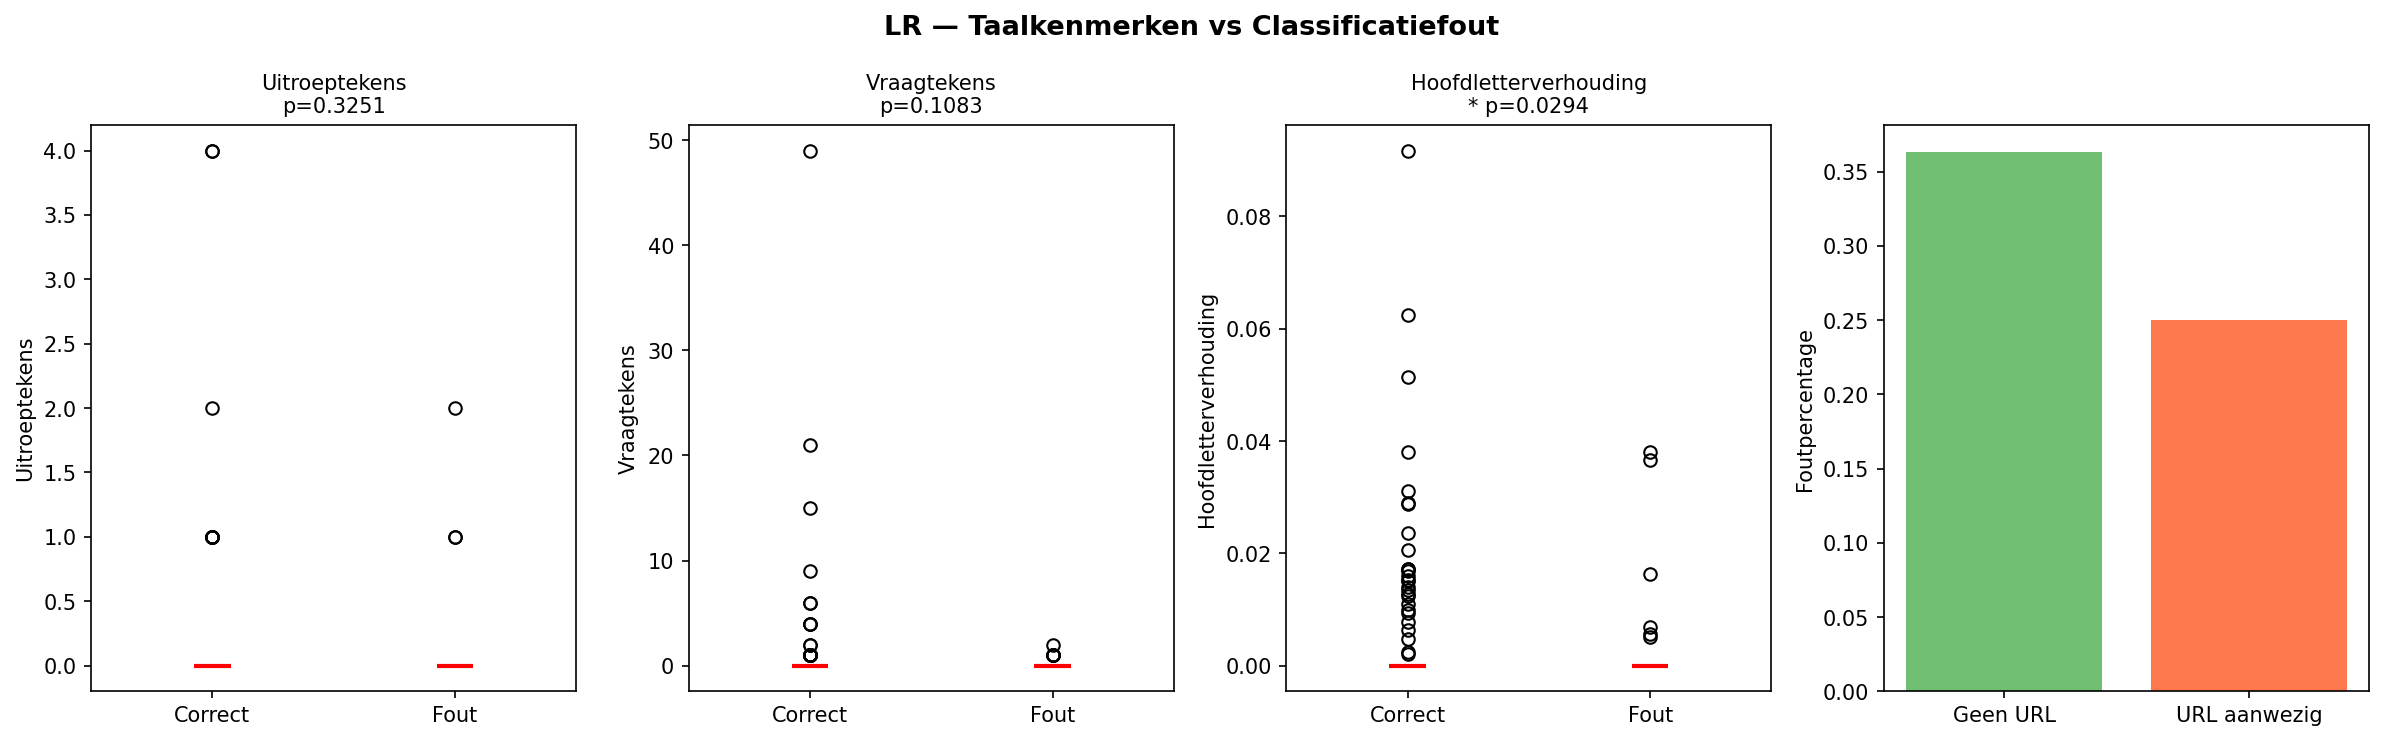
\includegraphics[width=0.75\textwidth]{../results/figures/taalgebruik_lr.png}
\caption{Top kenmerken voor Logistic Regression (waar/onwaar)}
\label{fig:lr_features}
\end{figure}

\section{SVM: Support Vector Machine}

\textbf{Bestand}: \texttt{src/models/train\_svm.py}

SVM is geselecteerd omdat het sterke theoretische garanties biedt voor
hoge-dimensionale, sparse feature-ruimtes zoals TF-IDF. Dit model is in de
literatuur een gebruikelijke keuze voor tekstclassificatie en vormt een goed
contrast met de lineaire LR-baseline en het semantische BERT-model.

\begin{lstlisting}[language=Python, basicstyle=\ttfamily\scriptsize,
  caption={SVM training pipeline with probabilistic calibration},
  literate={_}{\_}1]
from sklearn.svm import LinearSVC
from sklearn.calibration import CalibratedClassifierCV
from sklearn.pipeline import Pipeline
from sklearn.feature_extraction.text import TfidfVectorizer

pipeline = Pipeline([
    ('tfidf', TfidfVectorizer(
        max_features=50000, ngram_range=(1, 2),
        min_df=2, max_df=0.95, sublinear_tf=True
    )),
    ('svm', CalibratedClassifierCV(
        LinearSVC(C=1.0, class_weight='balanced', max_iter=10000)
    ))
])

pipeline.fit(X_train, y_train)
y_pred = pipeline.predict(X_test)
y_proba = pipeline.predict_proba(X_test)[:, 1]
\end{lstlisting}

De \texttt{Pipeline} combineert opnieuw TF-IDF met een classifier. \texttt{LinearSVC}
wordt gebruikt in plaats van de standaard \texttt{SVC} omdat het veel sneller is
voor grote, sparse datasets. \texttt{LinearSVC} werkt goed met de hoge-dimensionale
word-vectoren die uit TF-IDF voortkomen.

\texttt{CalibratedClassifierCV} wikkelt de SVM in een calibratiemodel. Een
klassieke SVM kan wel een klasse-label voorspellen (waar/onwaar), maar geeft
niet altijd betrouwbare kansschattingen. Door calibratie te gebruiken
kunnen we \texttt{predict\_proba} oproepen en AUC-ROC berekenen, wat belangrijk is
voor de evaluatie van mispredicties in plaats van alleen accuracy.

\texttt{class\_weight='balanced'} compenseert de ongelijke verdeling tussen de
labels en zorgt ervoor dat het model niet alleen focust op de meerderheidsklasse.

\section{BERT: Transformers}

\textbf{Bestand}: \texttt{src/models/train\_bert.py}

Model: \texttt{bert-base-uncased} (12 lagen, 768 hidden, 110M parameters)

\begin{lstlisting}[language=Python, basicstyle=\ttfamily\scriptsize,
  caption={BERT model fine-tuning script},
  literate={_}{\_}1]
from transformers import AutoTokenizer, AutoModelForSequenceClassification
from transformers import Trainer, TrainingArguments

tokenizer = AutoTokenizer.from_pretrained('bert-base-uncased')
model = AutoModelForSequenceClassification.from_pretrained(
    'bert-base-uncased', num_labels=2)

# Tokenisatie
def tokenize_function(examples):
    return tokenizer(examples['text'],
        padding='max_length', truncation=True, max_length=128)

train_dataset = train_dataset.map(tokenize_function, batched=True)
val_dataset = val_dataset.map(tokenize_function, batched=True)

# Training
training_args = TrainingArguments(
    output_dir='./results/bert/best_model',
    num_train_epochs=4,
    per_device_train_batch_size=16,
    learning_rate=2e-5,
    warmup_ratio=0.1,
    weight_decay=0.01,
    metric_for_best_model='f1',
    load_best_model_at_end=True,
    eval_strategy='steps',
    save_steps=100,
    eval_steps=100,
)

trainer = Trainer(model=model, args=training_args,
    train_dataset=train_dataset, eval_dataset=val_dataset)
trainer.train()
\end{lstlisting}

BERT is gekozen omdat het de volledige woordvolgorde en context van een bericht
kan modelleren. Mastodon-berichten kunnen subtiele semantische signalen en
contextuele nuance bevatten die niet goed door eenvoudige bag-of-words
representaties worden vastgelegd.

De tokenisatie stap zet de ruwe tekst om in tokens die door het voorgetrainde
BERT-model begrepen worden. \texttt{padding='max\_length'} en
\texttt{truncation=True} zorgen ervoor dat alle inputs dezelfde lengte krijgen,
waardoor batches efficiënt verwerkt kunnen worden.

De trainingsinstellingen zijn gekozen om BERT met een relatief lage
learning rate en een korte finetuning te trainen. \texttt{load\_best\_model\_at\_end=True}
zorgt ervoor dat het beste model op basis van de F1-score wordt bewaard.

\textbf{GPU-optimalisatie}: halveer de
\texttt{per\_device\_train\_batch\_size} of verhoog gradient accumulation
steps wanneer er onvoldoende VRAM beschikbaar is.

\section{Hyperparameter-tuning}

Voor SVM en Logistic Regression:

\begin{verbatim}
python src/models/train_svm.py --grid-search
python src/models/train_logistic_regression.py --grid-search
\end{verbatim}

Voor BERT: experimenteer met learning rate en batch size in config.yaml.

% ══════════════════════════════════════════════════════════════════
\section{Uitvoering van de pipeline}\label{sec:uitvoering}
% ══════════════════════════════════════════════════════════════════

\section{Installatie}

\begin{verbatim}
# 1. Kloon de repository
git clone <repository-url>
cd misinformatie_detectie

# 2. Maak een virtuele omgeving aan
python -m venv venv
venv\Scripts\activate          # Windows
# source venv/bin/activate     # Linux/Mac

# 3. Installeer afhankelijkheden
pip install -r requirements.txt
pip install -e .

# 4. Kopieer .env.example en vul je token in
copy .env.example .env
\end{verbatim}

\section{Volledige pipeline uitvoeren}

\begin{verbatim}
# Volledige pipeline (inclusief Mastodon-verzameling)
python run_pipeline.py

# Zonder Mastodon (gelabeld bestand al aanwezig)
python run_pipeline.py --skip-mastodon

# Zonder BERT (sneller, alleen SVM + LR)
python run_pipeline.py --skip-mastodon --skip-bert

# Met grid search voor hyperparameter-optimalisatie
python run_pipeline.py --skip-mastodon --grid-search

# Alleen evaluatie (modellen al getraind)
python run_pipeline.py --eval-only
\end{verbatim}

\section{Individuele stappen uitvoeren}

\begin{verbatim}
# Stap 1a: LIAR verwerken
python src/preprocessing/liar_preprocessor.py

# Stap 1b: Mastodon-berichten verzamelen
python src/preprocessing/mastodon_collector.py

# Stap 1c: Datasets samenvoegen
python src/preprocessing/data_merger.py

# Stap 2a: SVM trainen
python src/models/train_svm.py

# Stap 2b: Logistic Regression trainen
python src/models/train_logistic_regression.py

# Stap 2c: BERT fine-tunen
python src/models/train_bert.py

# Stap 3: Eindevaluatie
python src/evaluation/evaluate_all.py

# Stap 4: Factoranalyse
python src/evaluation/factor_analysis.py
\end{verbatim}

\section{Gegenereerde uitvoerbestanden}

Na een volledige pipeline-run zijn de volgende bestanden beschikbaar:

\begin{table}[H]
\centering
\caption{Gegenereerde bestanden na pipeline-uitvoering}
\begin{tabular}{ll}
\toprule
\textbf{Bestand} & \textbf{Inhoud} \\
\midrule
\texttt{results/model\_comparison\_test.csv} & F1/precision/recall per model \\
\texttt{results/svm/svm\_model.joblib} & Getraind SVM-model \\
\texttt{results/svm/svm\_top\_features.csv} & Top-50 discriminerende kenmerken \\
\texttt{results/lr/lr\_model.joblib} & Getraind LR-model \\
\texttt{results/lr/lr\_top\_waar\_features.csv} & Top kenmerken voor klasse ``waar'' \\
\texttt{results/bert/best\_model/} & Beste BERT-checkpoint \\
\texttt{results/bert/bert\_training\_history.csv} & Verlies/F1 per epoch \\
\texttt{results/factor\_taalgebruik\_statistieken.csv} & Mann-Whitney U resultaten \\
\texttt{results/figures/*.png} & Alle grafieken en visualisaties \\
\bottomrule
\end{tabular}
\end{table}

\section{Reproduceerbaarheid en versiebeheer}
\label{sec:reproduceerbaarheid}
% ══════════════════════════════════════════════════════════════════

\subsection{Random seed}

Alle willekeurige processen (datasplitsing, modelinitialisatie, dataschudding)
gebruiken een vaste seed van \textbf{42}, ingesteld via de functie
\texttt{set\_seed()} in \texttt{src/utils.py}. Dit garandeert dat resultaten
volledig reproduceerbaar zijn.

\subsection{Git-versiebeheer}

De repository bevat een \texttt{.gitignore} die voorkomt dat gevoelige
bestanden (API-tokens in \texttt{.env}) of grote bestanden
(modelgewichten, ruwe dataset) worden gecommit.

Aanbevolen commitstrategie:

\begin{verbatim}
git add src/ notebooks/ config.yaml requirements.txt
git commit -m "feat: SVM baseline getraind (val F1=0.XX)"
\end{verbatim}

\subsection{Configuratiebeheer}

Alle hyperparameters en paden zijn gecentraliseerd in \texttt{config.yaml}.
Dit betekent dat experimenten kunnen worden herhaald of aangepast zonder
de broncode te wijzigen.

% ══════════════════════════════════════════════════════════════════
\chapter{Evaluatie en analyse}\label{ch:evaluatie}

\section{Evaluatiemetrieken}

Alle modellen worden beoordeeld op een onafhankelijke testset. Gebruikte
metrieken (berekend in \texttt{src/evaluation/metrics.py}):

\begin{table}[H]
\centering
\caption{Evaluatiemetrieken}
\begin{tabular}{ll}
\toprule
\textbf{Metriek} & \textbf{Beschrijving} \\
\midrule
Accuracy & \% correct geclassificeerde berichten \\
F1 (macro) & Harmonisch gemiddelde per klasse (aangewezen bij onbalans) \\
F1 (binary) & F1 voor klasse ``waar'' alleen \\
Precision & Van voorspelde ``waar'': \% echt waar \\
Recall & Van werkelijke ``waar'': \% correct geïdentificeerd \\
AUC-ROC & Discriminerend vermogen \\
\bottomrule
\end{tabular}
\end{table}

\section{Modelevaluatie}

Via \texttt{src/evaluation/evaluate\_all.py} worden gegenereerd:

\begin{verbatim}
python src/evaluation/evaluate_all.py
\end{verbatim}

\subsection{Metriekvergelijking}

\begin{figure}[H]
\centering
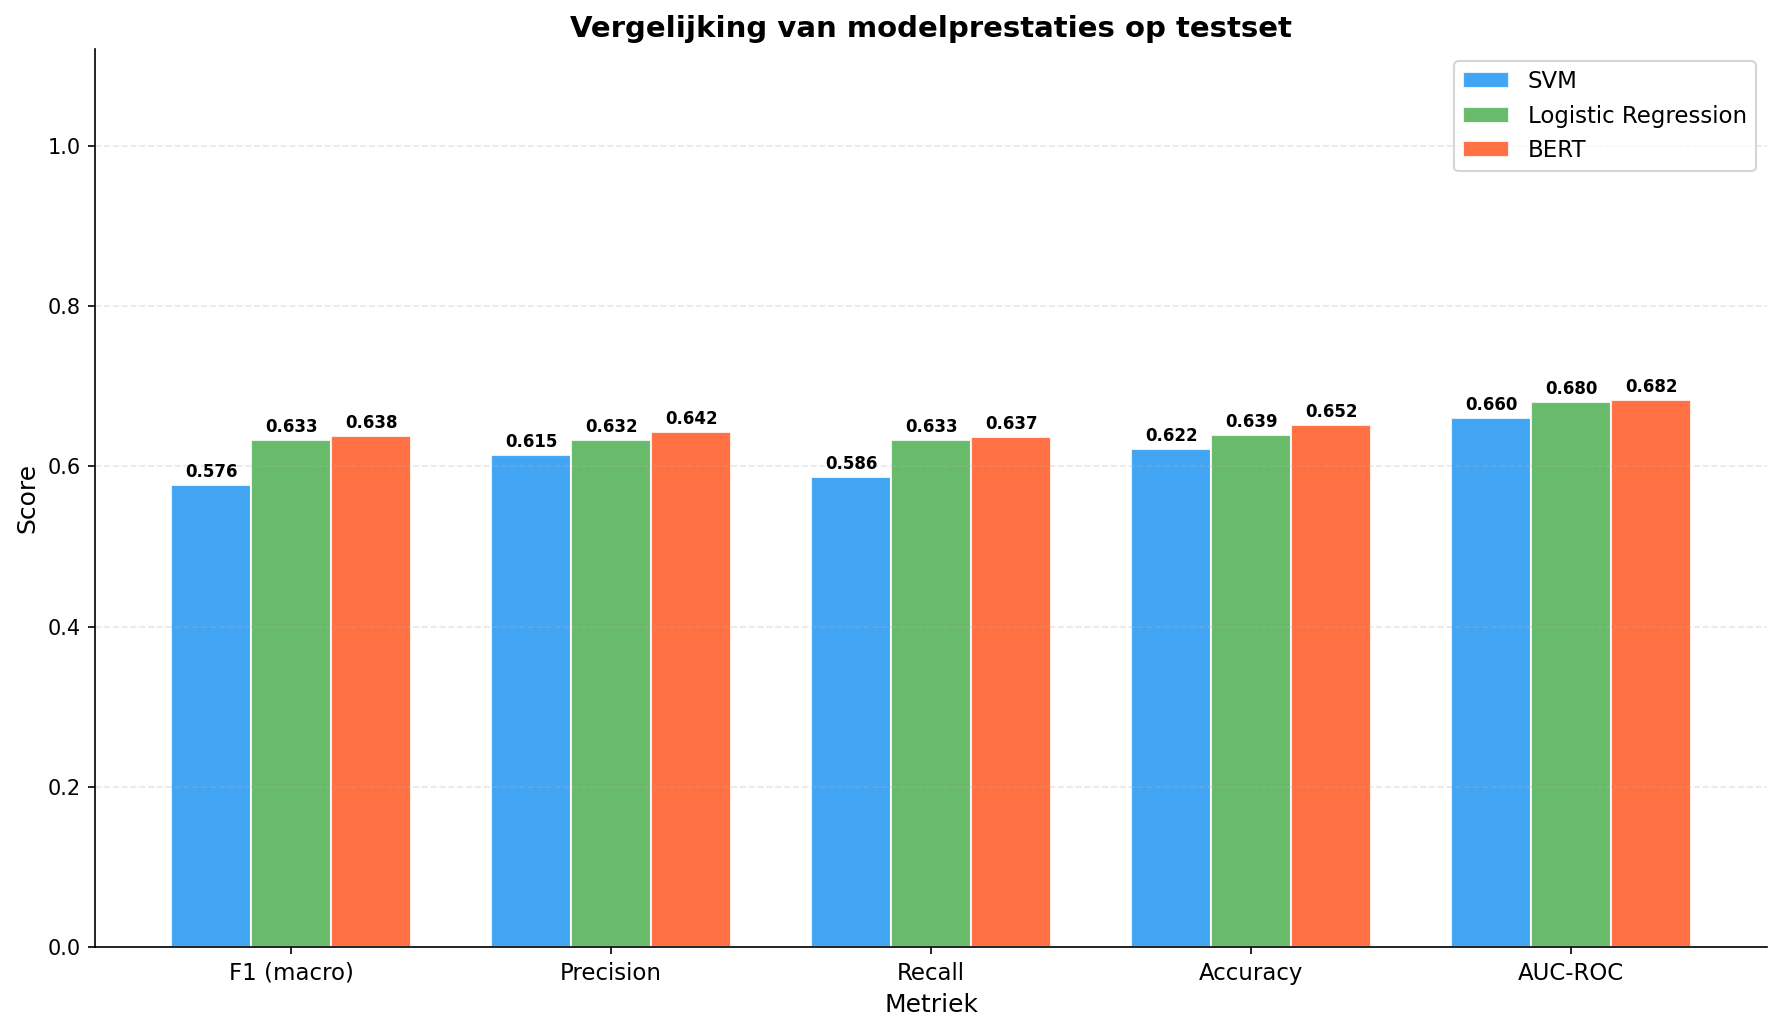
\includegraphics[width=0.8\textwidth]{../results/figures/metrics_comparison.png}
\caption{Vergelijking van F1, Precision, Recall en Accuracy per model (SVM, LR, BERT)}
\label{fig:metrics}
\end{figure}

\subsection{Verwarringsmatrices}

\begin{figure}[H]
\centering
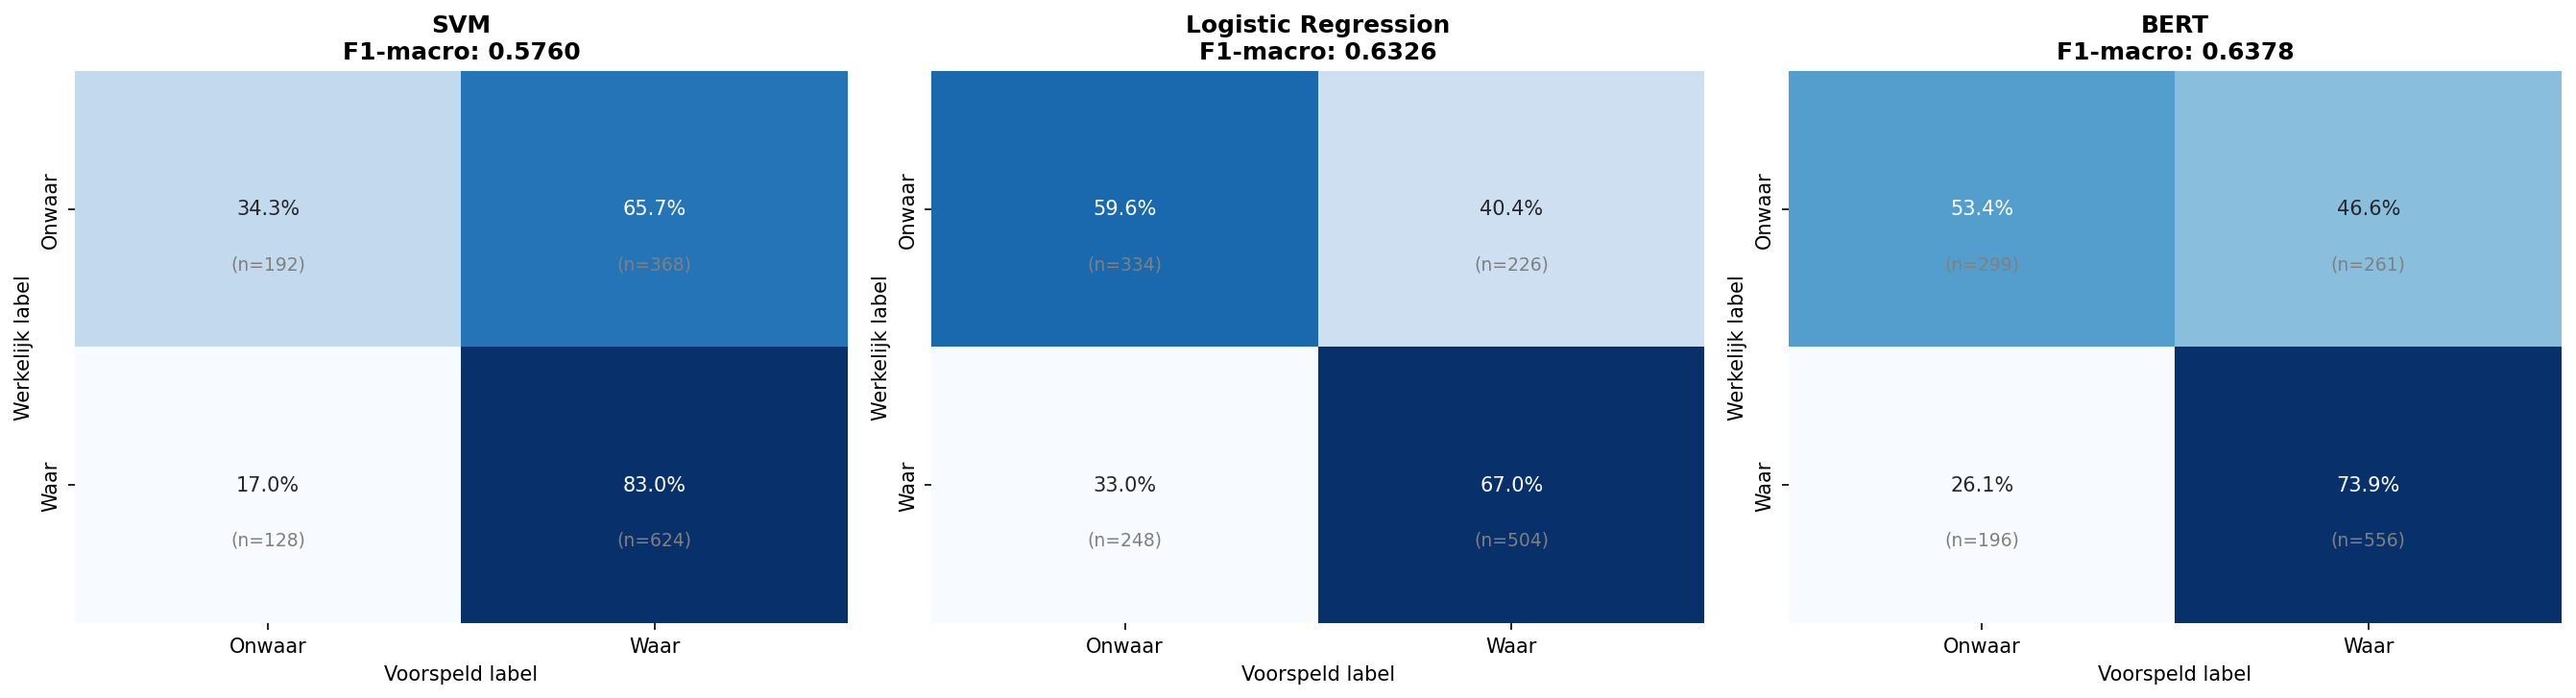
\includegraphics[width=0.85\textwidth]{../results/figures/confusion_matrices.png}
\caption{Verwarringsmatrices voor alle drie modellen op testset. Opmerking: metrieke labels in figuur verwijzen naar F1-macro (niet F2-macro).}
\label{fig:confusion}
\end{figure}

\subsection{ROC-curves}

\begin{figure}[H]
\centering
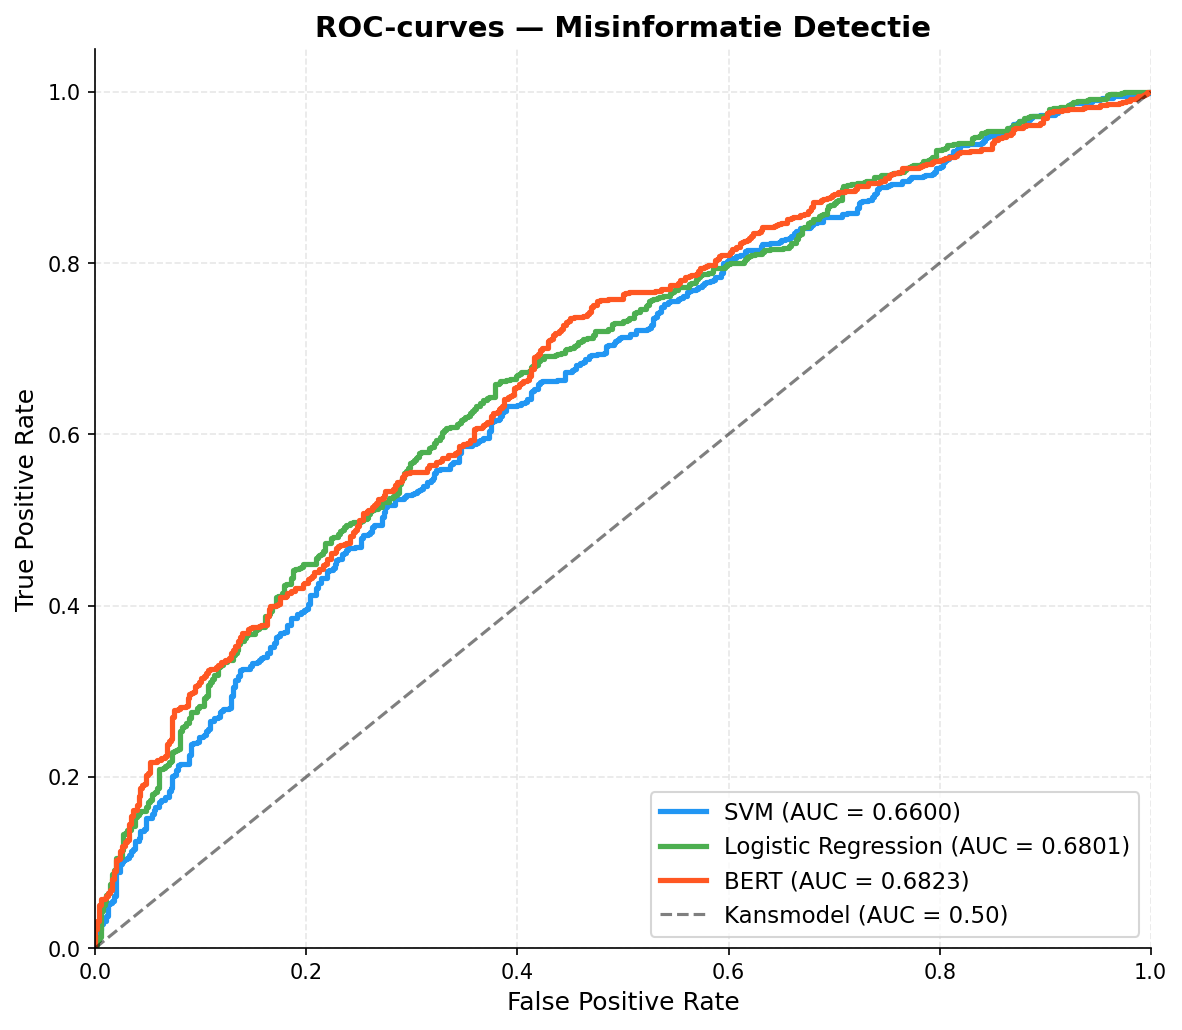
\includegraphics[width=0.75\textwidth]{../results/figures/roc_curves.png}
\caption{ROC-curves met AUC-scores per model}
\label{fig:roc}
\end{figure}

\begin{figure}[H]
\centering
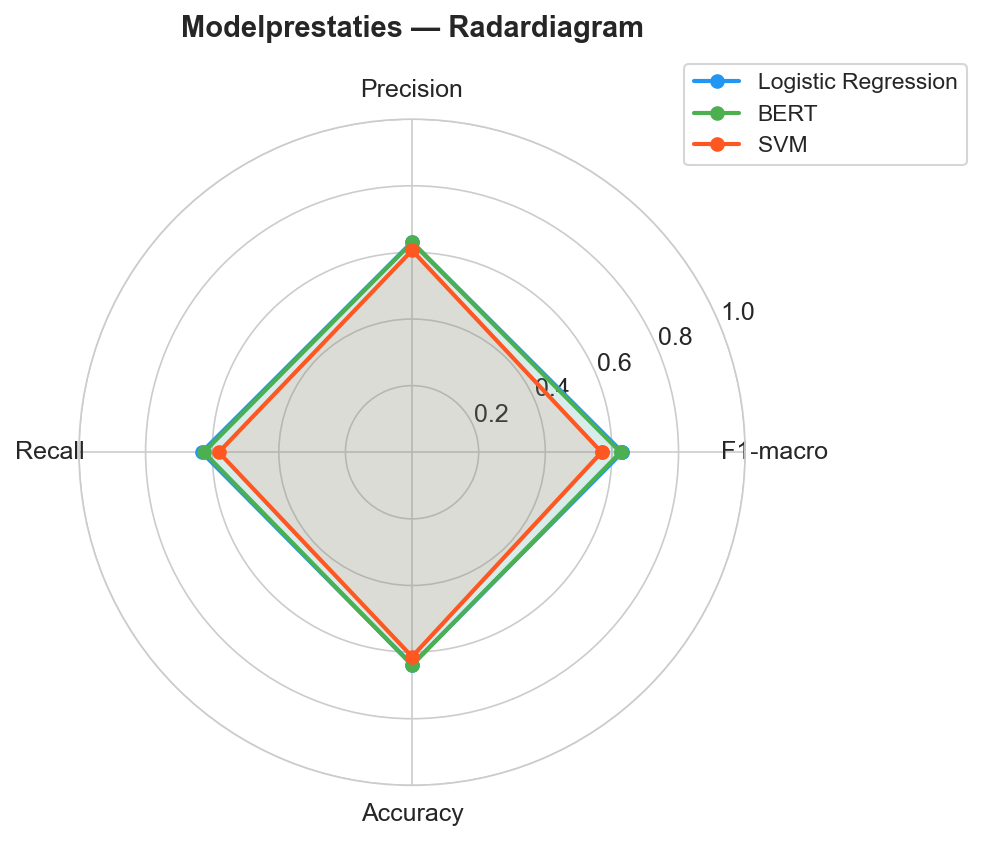
\includegraphics[width=0.7\textwidth]{../results/figures/radar_vergelijking.png}
\caption{Radardiagram van modelprestaties}
\label{fig:radar}
\end{figure}

\section{Factoranalyse}

Via \texttt{src/evaluation/factor\_analysis.py} worden:

\begin{verbatim}
python src/evaluation/factor_analysis.py
\end{verbatim}

\subsection{Factor 1: Berichtlengte}

Chi-square test (per lengtecategorie). Resultaten in \texttt{factor\_length\_analysis.csv}.

\begin{figure}[H]
\centering
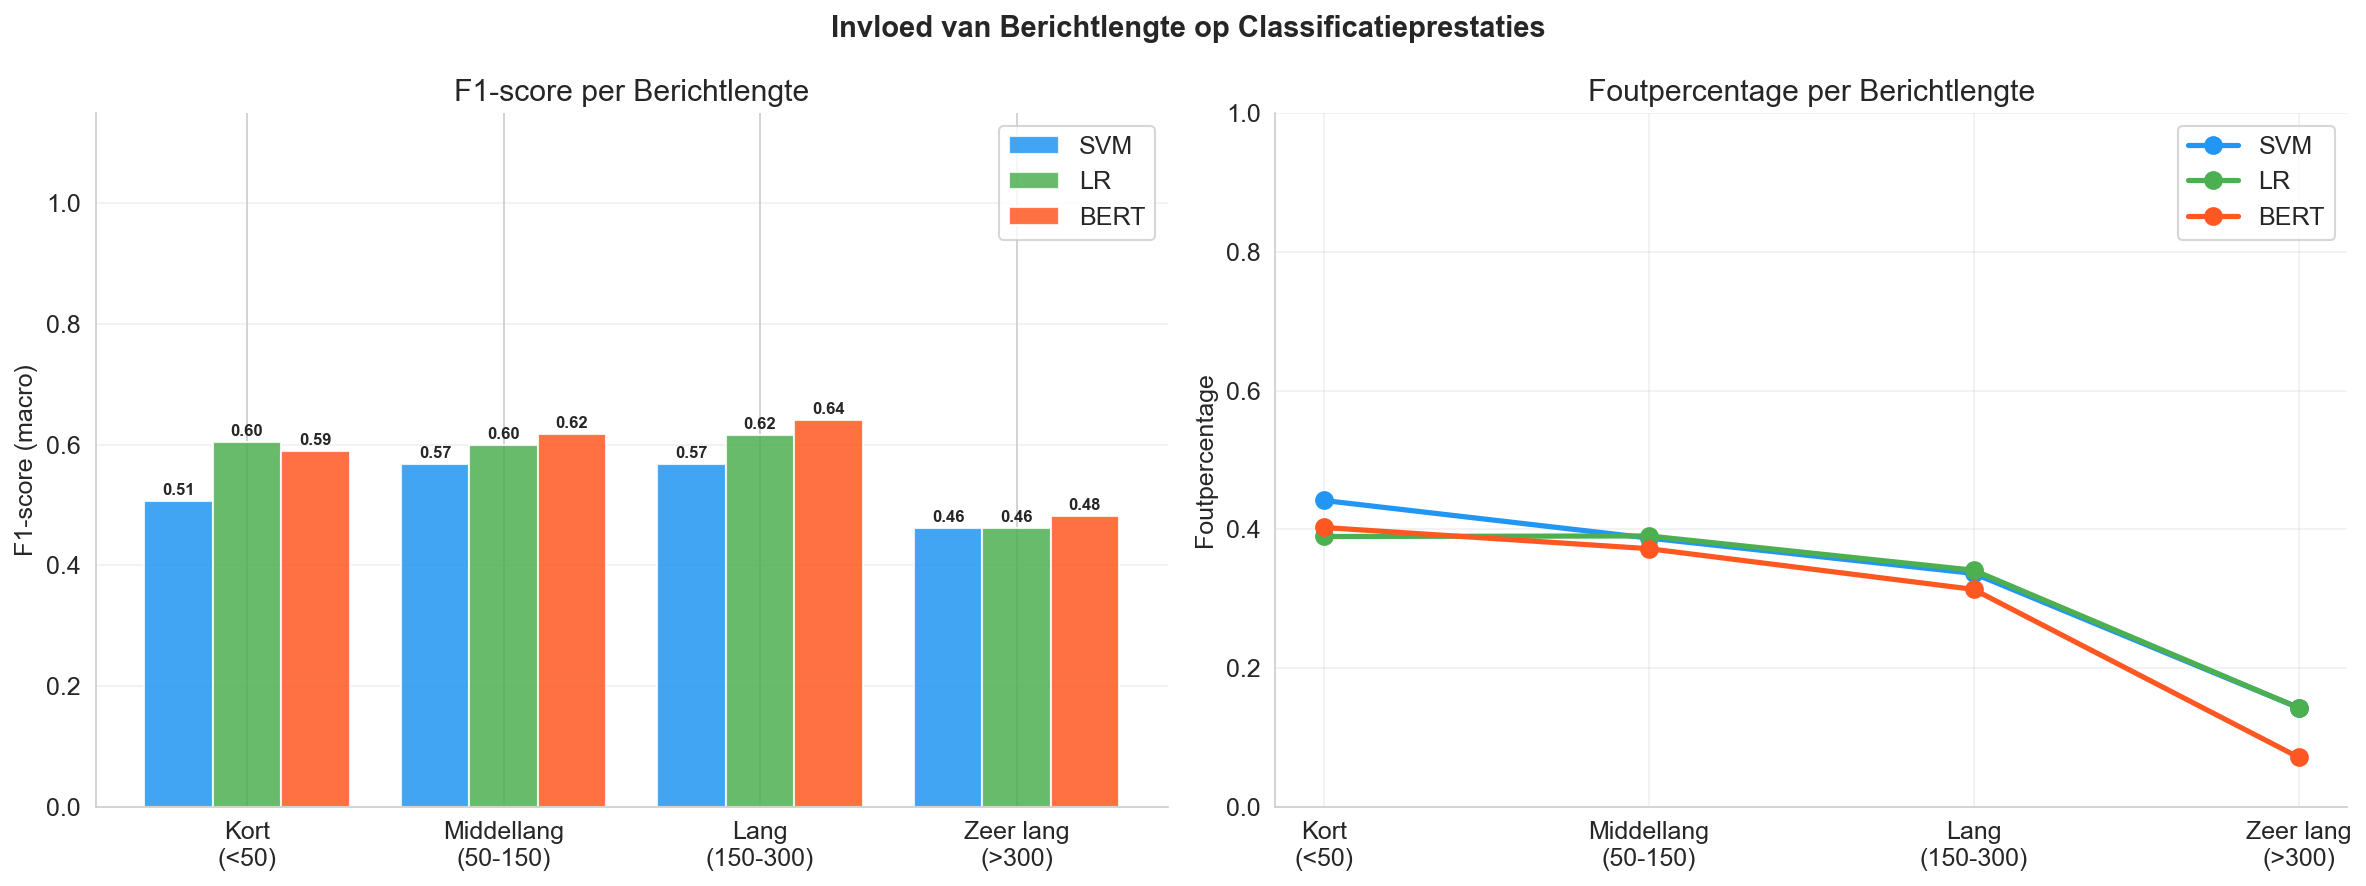
\includegraphics[width=0.75\textwidth]{../results/figures/analyse_berichtlengte.png}
\caption{Invloed van berichtlengte op classificatiefout per model}
\label{fig:length}
\end{figure}

\subsection{Factor 2: Bronbetrouwbaarheid}

ANOVA (laag/middel/hoog). Resultaten in \texttt{factor\_trust\_analysis.csv}.

\begin{figure}[H]
\centering
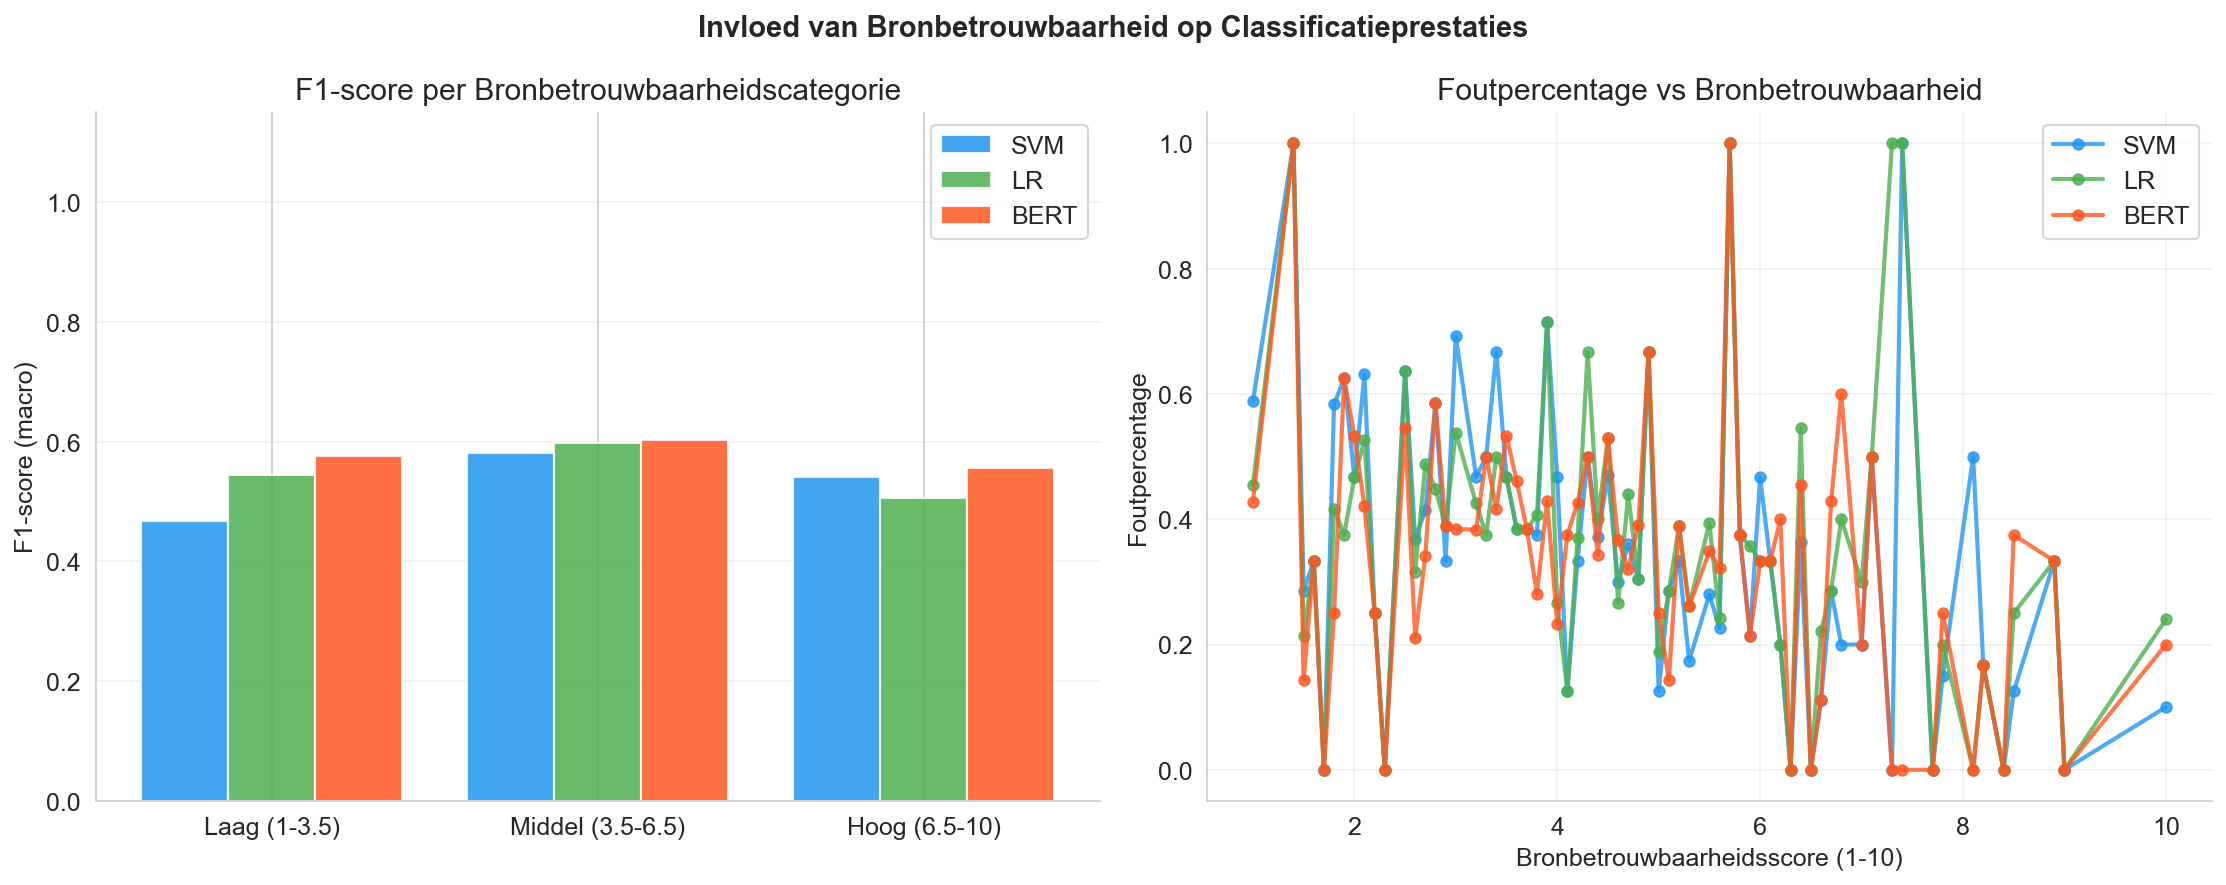
\includegraphics[width=0.75\textwidth]{../results/figures/analyse_bronbetrouwbaarheid.png}
\caption{Invloed van bronbetrouwbaarheid op modelprestaties}
\label{fig:trust}
\end{figure}

\subsection{Factor 3: Taalgebruik}

Mann-Whitney U toets voor exclamatie's, vragen, CAPS, URLs.
Resultaten in \path{factor_taalgebruik_statistieken.csv}.

\begin{figure}[H]
\centering
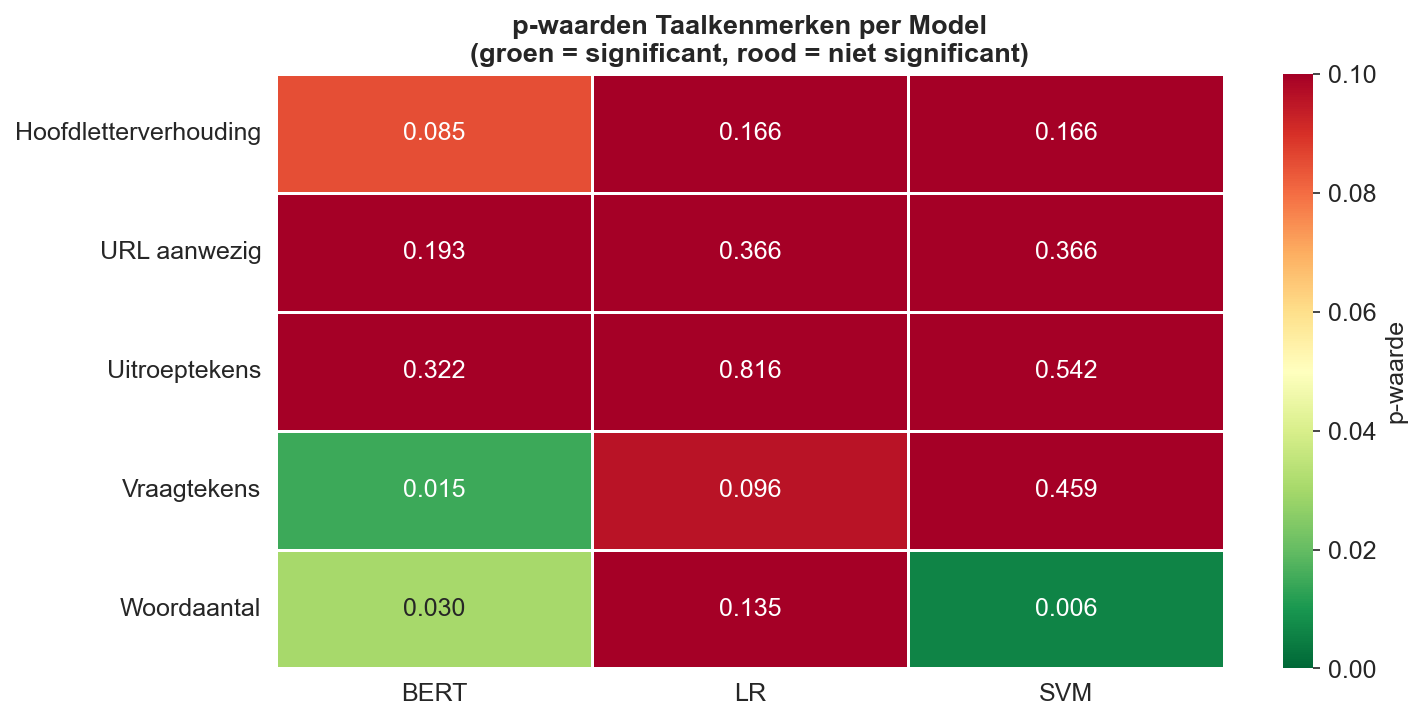
\includegraphics[width=0.8\textwidth]{../results/figures/heatmap_taalkenmerken.png}
\caption{Heatmap van p-waarden voor taalgebruikskenmerken (SVM en LR)}
\label{fig:linguistic}
\end{figure}

\section{Analyse Jupyter Notebook}

Volledige visualisatie in \texttt{notebooks/02\_analyse\_rapport.ipynb}.
Enkele belangrijke figuren:

\subsection{BERT trainingsverloop}

\begin{figure}[H]
\centering
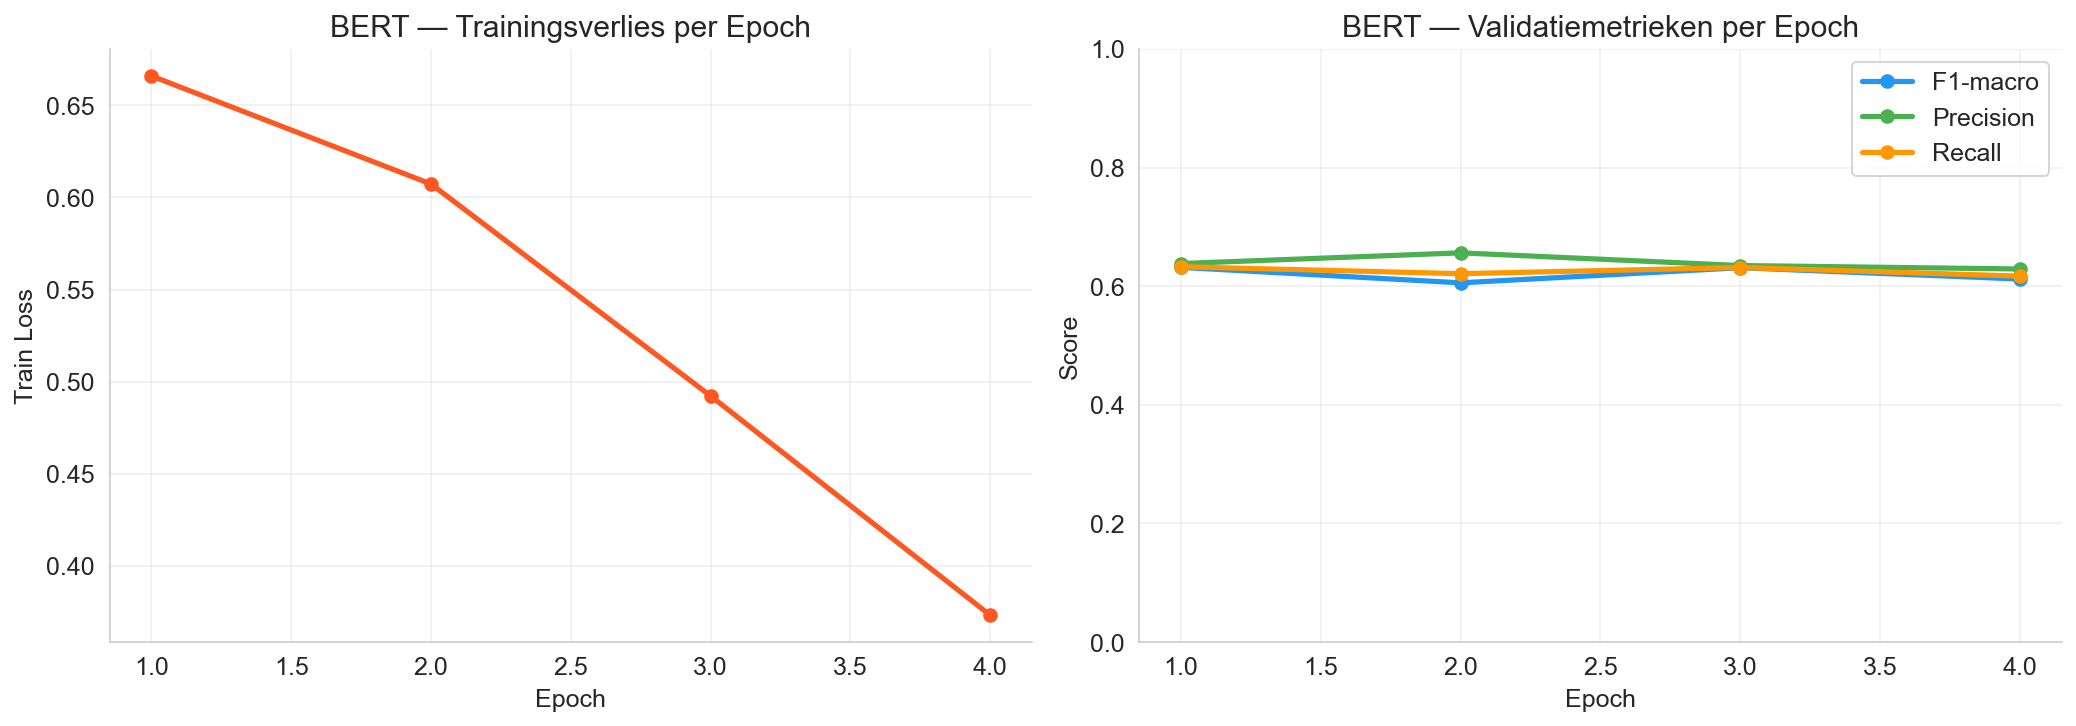
\includegraphics[width=0.75\textwidth]{../results/figures/bert_trainingsverloop.png}
\caption{Trainings- en validatieverlies + F1-macro per epoch}
\label{fig:bert}
\end{figure}

\subsection{F1-score per berichtlengte}

\begin{figure}[H]
\centering
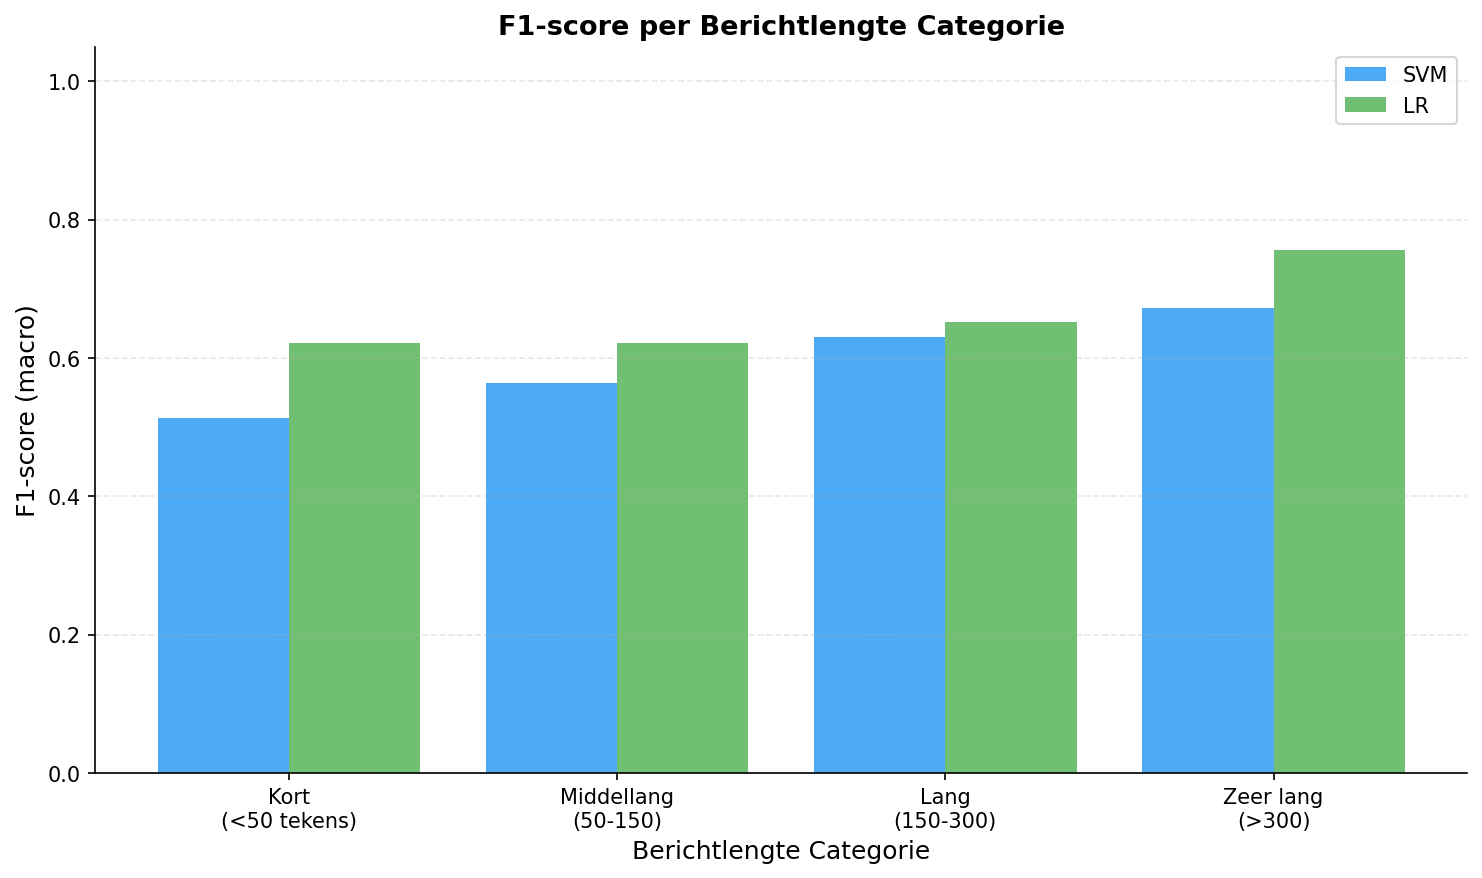
\includegraphics[width=0.75\textwidth]{../results/figures/f1_per_lengte.png}
\caption{Modelprestaties uitgesplitst naar berichtlengte}
\label{fig:f1length}
\end{figure}

\subsection{Exploratieve data-analyse}

Zie ook \texttt{notebooks/01\_eda.ipynb} voor labelbalans, wordclouds en correlatiematrices:

\begin{figure}[H]
\centering
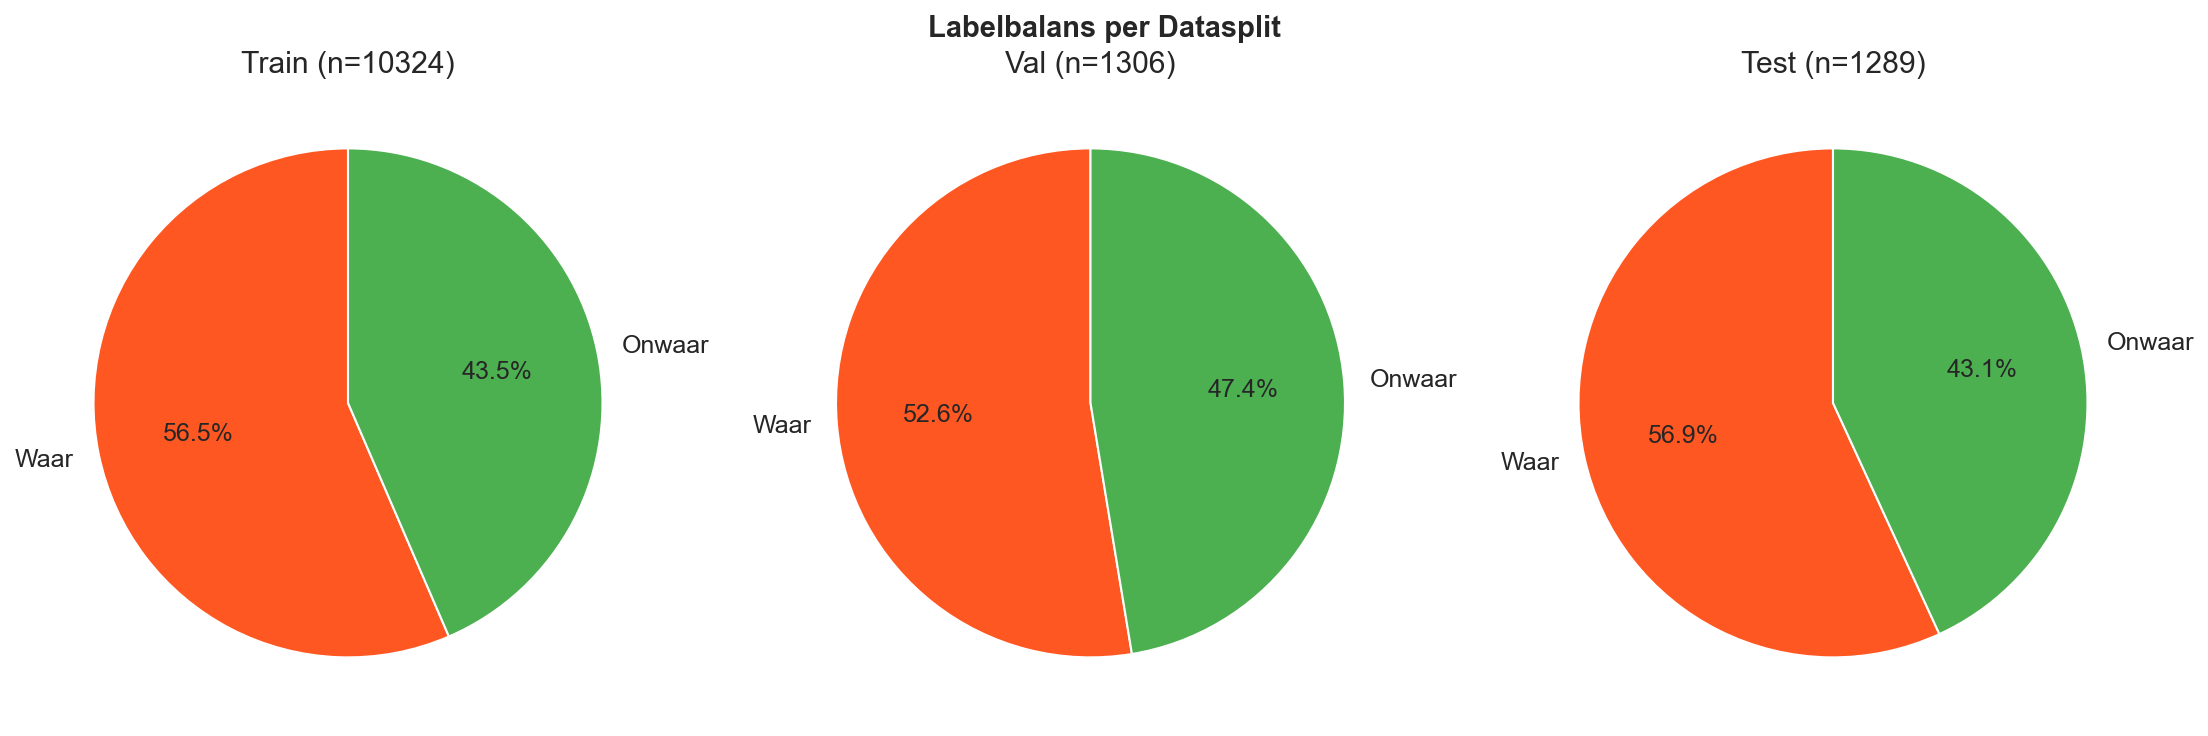
\includegraphics[width=0.75\textwidth]{../results/figures/eda_labelbalans.png}
\caption{Balans van waar/onwaar berichten in dataset}
\label{fig:balance}
\end{figure}


}{
    \chapter{Productdocumentatie}
    \textit{Let op: bestand product.tex niet gevonden.}
}

% 4. Resultaten (Nog te doen)
% \input{resultaten} 

% 5. Conclusie (Nog te doen)
% \input{conclusie} 

% 6. Algemeen Besluit en Discussie
\IfFileExists{06_algemeen_besluit.tex}{
    % Hoofdstuk 6: Algemeen besluit en discussie
\chapter{Algemeen Besluit en Discussie}
\label{cha:algemeen_besluit}

\section{Conclusie en Beantwoording van de Onderzoeksvragen}
Dit onderzoek had als centrale vraag: "Welke machine learning modellen zijn het meest geschikt voor het detecteren van misinformatie op Mastodon en welke inhoudelijke factoren beïnvloeden de nauwkeurigheid?"

Het antwoord op deze vraag is genuanceerd. Zoals de resultaten aantonen, leveren transformer‑gebaseerde modellen zoals BERT de beste automatische detectieprestaties op tekstuele Mastodon‑berichten. Tegelijkertijd bewijst een eenvoudigere lineaire benadering zoals Logistic Regression een verrassend sterke en praktisch bruikbare baseline te vormen. Dit sluit direct aan bij de bevindingen van \textcite{pelrine2021surprising}, die in hun werk eveneens de onverwacht sterke prestaties van zulke compacte baselines aantonen. Daarnaast blijkt uit de statistische analyses dat zowel de tekstuele inhoud, de stilistische kenmerken als de bronmetadata de classificatienauwkeurigheid substantieel beïnvloeden. Dit bevestigt tevens de theoretische risico's die naar voren worden gebracht in het werk van \textcite{Zia2025} omtrent de complexiteit en de limieten van geautomatiseerde moderatie binnen het heterogene Fediverse.

Samenvatting van modelprestaties:
\begin{itemize}
  \item \textbf{BERT}: overall het meest geschikt; $\text{accuracy} = 0{,}652$, macro $F_1 = 0{,}638$, binaire $F_1 = 0{,}709$ en $\text{AUC‑ROC} = 0{,}682$. Deze resultaten ondersteunen dat het bidirectionele semantische begrip van BERT beter generaliseert naar nieuwe, onbekende berichten en subtiele contextuele signalen oppikt, een mechanisme dat diepgaand is beschreven door \textcite{Devlin2019}.
  \item \textbf{Logistic Regression}: een compacte en transparante baseline met sterke prestaties ($\text{accuracy} = 0{,}639$, macro $F_1 = 0{,}633$). Het succes van deze aanpak onderstreept de argumentatie van \textcite{pelrine2021surprising} dat traditionele statistische modellen in veel NLP-taken een competitief en computationeel efficiënt alternatief blijven voor deep learning.
  \item \textbf{SVM}: presteerde lager ($\text{accuracy} = 0{,}622$, macro $F_1 = 0{,}576$), hoewel het een hoge recall voor de klasse "waar" rapporteerde ($\text{recall} = 0{,}830$). Dit wijst op een bias richting de correcte identificatie van waarheidsgetrouwe berichten, ten koste van de balans tussen de klassen.
\end{itemize}

Beantwoording van deelvragen:
\begin{itemize}
  \item \textbf{Welk model is het meest geschikt?} BERT geniet de voorkeur voor optimale detectieprestaties; Logistic Regression dient als een realistisch en computationeel efficiënt alternatief voor resource‑beperkte omgevingen, zoals eveneens geëvalueerd door \textcite{Khatri2025}.
  \item \textbf{Welke inhoudelijke factoren beïnvloeden de nauwkeurigheid?} Berichtlengte, bronbetrouwbaarheid en specifieke taalgebruikskenmerken (zoals vraagtekens en het totale woordaantal) beïnvloeden de nauwkeurigheid significant.
  \item \textbf{Hoe goed generaliseert transfer learning?} Zero‑shot transfer van de Amerikaanse, politiek getinte LIAR‑dataset, oorspronkelijk gedocumenteerd door \textcite{Wang2017}, leverde bruikbare signalen op voor Mastodon, maar de beperkte handgelabelde testset van 300 Mastodon‑berichten (gevalideerd via VRT NWS Factcheck og PolitiFact) beperkt de statistische zekerheid van een bredere generalisatie.
\end{itemize}

\subsection{Invloed van inhoudelijke factoren}
Op basis van de uitgevoerde statistische toetsen concluderen we het volgende:
\begin{itemize}
  \item \textbf{Berichtlengte (Chi‑square test)}: langere berichten leiden vaker tot classificatiefouten, wat wijst op moeilijkheden bij het ontleden van complexe of gelaagde claims in vergelijking met kortere segmenten.
  \item \textbf{Bronbetrouwbaarheid (ANOVA)}: berichten met een lage bronbetrouwbaarheid werden significant moeilijker correct geclassificeerd, wat de noodzaak onderstreept om externe reputatie-indicatoren te integreren.
  \item \textbf{Taalgebruikskenmerken (Mann‑Whitney U)}: vraagtekens waren een statistisch significante indicator ($p = 0{,}015$ voor BERT); het woordaantal was eveneens significant voor zowel BERT ($p = 0{,}030$) als SVM ($p = 0{,}006$). Uitroeptekens en de hoofdletterverhouding bleken daarentegen niet‑significant. Conclusie: zowel tekstinhoud als stijlkenmerken bevatten belangrijke detectiesignalen, maar niet alle oppervlakkige stilistische kenmerken zijn standvastig.
\end{itemize}

\section{Discussie en Beperkingen van het Onderzoek}
Er zijn meerdere beperkingen en overwegingen die de interpretation van de resultaten nuanceren.

\subsection{Datagrootte and domain shift}
De toepassing van zero‑shot transfer learning van de Amerikaanse, politiek getinte LIAR‑dataset naar het Mastodon‑domein bleek succesvol in het genereren van bruikbare modellen. Tegelijkertijd is de handmatig gelabelde testset van 300 Mastodon‑berichten (gevalideerd via VRT NWS Factcheck en PolitiFact) relatief klein, waardoor betrouwbaarheidsmarges en generaliseerbaarheid beperkt blijven. Toekomstig werk moet grotere, representatievere Mastodon‑datasets verzamelen om de invloed van platform-specifiek taalgebruik beter te ondervangen, een probleem dat ook door \textcite{castillo2011information} en \textcite{perez2018automatic} vroegtijdig werd opgemerkt.

\subsection{De intentie‑paradox}
Zoals \textcite{wardle2017information} accuraat uiteenzetten, is het onderscheid tussen misinformatie (onbedoeld onjuist) en desinformatie (opzettelijk misleidend) in essentie een kwestie van intentie — iets wat text‑only modellen niet rechtstreeks kunnen afleiden. Onze modellen detecteren tekstuele onjuistheden of veronderstelde misleidende patronen, maar kunnen geen interne intentie van de auteur meten.

\subsection{Rekenintensiteit versus decentralisatie}
Hoewel BERT de beste prestaties biedt, brengt het aanzienlijke training‑ en inferencekosten met zich mee, een nadeel dat ook door \textcite{Khatri2025} wordt onderstreept. In het Fediverse, waar veel Mastodon‑instances beperkte financiële en technische middelen hebben, kan dit een belemmering vormen. Logistic Regression biedt hierdoor een praktisch uitvoerbaar en goedkoper alternatief met een betere transparantie voor decentrale architecturen.

\section{Praktische Implicaties en Succesreflectie}
Het project is geslaagd in het aantonen dat automatische misinformatiedetectie in een decentrale omgeving haalbaar is zonder centrale autoriteit. Belangrijke praktische consequenties:
\begin{itemize}
  \item Geautomatiseerde pre‑screening kan moderators ondersteunen door prioriteiten te stellen en signalen te markeren, waardoor vrijwillige moderators minder overbelast raken binnen de gedistribueerde structuren die \textcite{Zia2025} omschrijven.
  \item Een hybride aanpak is aan te raden: zware modellen (BERT) kunnen op dedicated nodes of gecentraliseerde diensten draaien, terwijl lichtere modellen (Logistic Regression) lokaal op kleine instances kunnen draaien om snelle, interpreteerbare signalen te leveren.
\end{itemize}

\section{Aanbevelingen voor Verder Onderzoek}
Drie concrete, technisch onderbouwde richtingen:
\begin{enumerate}
  \item \textbf{Multimodale Detectie:} breid het systeem uit naar beeld‑ en videoanalyse, bijvoorbeeld door CLIP‑achtige architecturen te integreren, aangezien misinformatie vaak multimodaal is, zoals \textcite{zhou2020similarity} benadrukken.
  \item \textbf{Explainable AI (XAI):} integreer technieken zoals LIME of SHAP om het "black box"‑karakter van deep learning te verminderen en moderatoren exact te tonen welke woorden of frasen bijdroegen aan een "onwaar"‑label.
  \item \textbf{Contextuele en Netwerkkenmerken:} verrijk tekstuele modellen met metadata en netwerkinformatie (zoals de defederatie‑historiek en serverreputatie) om claims in hun breder sociale context te plaatsen, in lijn met de moderatiestructuur van het Fediverse.
\end{enumerate}

\section{Slotopmerking}
De resultaten tonen dat technische hulpmiddelen een waardevolle rol kunnen spelen in het ondersteunen van gedistribueerde moderatie op Mastodon. BERT levert de hoogste prestaties, Logistic Regression is praktisch en interpreteerbaar, en inhoudelijke plus netwerkcontext zijn essentieel voor robuuste detectie. Verdere schaalvergroting van de dataset en de integratie van multimodale en explainable technieken vergroten de praktische toepasbaarheid van zulke systemen aanzienlijk.
}{
    % Let op: bestand 06_algemeen_besluit.tex niet gevonden.
}

%---------- Bijlagen -----------------------------------------------------------

\appendix

\chapter{Bijlage: Volledige bestandslijst}
\label{ch:bijlage-bestandslijst}
\begin{longtable}{lp{8cm}}
\toprule
\textbf{Bestand} & \textbf{Functie} \\
\midrule
\endhead
\texttt{run\_pipeline.py} & Hoofdscript; orkestreert de volledige pipeline \\
\texttt{config.yaml} & Centrale configuratie voor alle parameters en paden \\
\texttt{requirements.txt} & Python-pakketafhankelijkheden \\
\texttt{setup.py} & Installatiebestand voor lokale pakketimport \\
\texttt{.env.example} & Template voor API-tokens (nooit committen) \\
\texttt{.gitignore} & Uitsluitingen voor Git \\
\texttt{src/utils.py} & Hulpfuncties: config laden, logging, seed, apparaat \\
\texttt{src/preprocessing/mastodon\_collector.py} & Mastodon API-verzameling \\
\texttt{src/preprocessing/liar\_preprocessor.py} & LIAR-dataset verwerking \\
\texttt{src/preprocessing/data\_merger.py} & Samenvoegen LIAR + Mastodon \\
\texttt{src/models/train\_svm.py} & SVM training en grid search \\
\texttt{src/models/train\_logistic\_regression.py} & LR training en grid search \\
\texttt{src/models/train\_bert.py} & BERT fine-tuning \\
\texttt{src/evaluation/metrics.py} & F1, precision, recall, AUC-ROC \\
\texttt{src/evaluation/evaluate\_all.py} & Eindevaluatie op testset \\
\texttt{src/evaluation/factor\_analysis.py} & Chi-kwadraat, ANOVA, Mann-Whitney U \\
\texttt{tests/test\_preprocessing.py} & 20+ unittests \\
\texttt{notebooks/01\_eda.ipynb} & Exploratieve data-analyse \\
\texttt{notebooks/02\_analyse\_rapport.ipynb} & Volledige scriptie-analyse \\
\bottomrule
\end{longtable}

\chapter{Onderzoeksvoorstel}
\label{ch:onderzoeksvoorstel}

Het onderwerp van deze bachelorproef is gebaseerd op een onderzoeksvoorstel dat vooraf werd beoordeeld door de promotor. Dat voorstel is opgenomen in deze bijlage.

%% TODO: 
%\section*{Samenvatting}

% Kopieer en plak hier de samenvatting (abstract) van je onderzoeksvoorstel.

% Verwijzing naar het bestand met de inhoud van het onderzoeksvoorstel
\input{../voorstel/voorstel-inhoud}

%%---------- Andere bijlagen --------------------------------------------------
% TODO: Voeg hier eventuele andere bijlagen toe. Bv. als je deze BP voor de
% tweede keer indient, een overzicht van de verbeteringen t.o.v. het origineel.
%\input{...}

%%---------- Backmatter, referentielijst ---------------------------------------

\backmatter{}

\setlength\bibitemsep{2pt} %% Add Some space between the bibliograpy entries
\printbibliography[heading=bibintoc]

\end{document}
